%% Преамбула TeX-файла

% 1. Стиль и язык
\documentclass[utf8x, 12pt]{G7-32} % Стиль (по умолчанию будет 14pt)

% Остальные стандартные настройки убраны в preamble-std.tex
\sloppy

% 1. Настройки стиля ГОСТ 7-32
% Для начала определяем, хотим мы или нет, чтобы рисунки и таблицы нумеровались в пределах раздела, или нам нужна сквозная нумерация.
% А не забыл ли автор букву 't' ?
\EqInChapter % формулы будут нумероваться в пределах раздела
\TableInChapter % таблицы будут нумероваться в пределах раздела
\PicInChapter % рисунки будут нумероваться в пределах раздела

% 2. Добавляем гипертекстовое оглавление в PDF
\usepackage[
bookmarks=true, colorlinks=true, unicode=true,
urlcolor=black,linkcolor=black, anchorcolor=black,
citecolor=black, menucolor=black, filecolor=black,
]{hyperref}

% 3. Изменение начертания шрифта --- после чего выглядит таймсоподобно.
% apt-get install scalable-cyrfonts-tex

\IfFileExists{cyrtimes.sty}
    {
        \usepackage{cyrtimespatched}
    }
    {
        % А если Times нету, то будет CM...
    }


% 4. Прочие полезные пакеты.
\usepackage{underscore} % Ура! Теперь можно писать подчёркивание.
                        % И нельзя использовать подчёркивание в файлах.
                        % Выбирай, но осторожно.

\usepackage{graphicx}   % Пакет для включения рисунков

 % 5. Любимые команды
\newcommand{\Code}[1]{\textbf{#1}}

% 6. Поля
% С такими оно полями оно работает по-умолчанию:
% \RequirePackage[left=20mm,right=10mm,top=20mm,bottom=20mm,headsep=0pt]{geometry}
% Если вас тошнит от поля в 10мм --- увеличивайте до 20-ти, ну и про переплёт не забывайте:
\geometry{right=20mm}
\geometry{left=30mm}


% 7. Tikz
\usepackage{tikz}
\usetikzlibrary{arrows,positioning,shadows}

% ER diagramm
\usepackage{tikz-er2}
\usepackage{graphicx}

% UML sequences
\usepackage[underline=true,rounded corners=false]{pgf-umlsd}

%многостраничные таблицы
\usepackage{longtable}
% 8 Листинги

\usepackage{listings}

% Значения по умолчанию
\lstset{
  basicstyle= \footnotesize,
  breakatwhitespace=true,% разрыв строк только на whitespacce
  breaklines=true,       % переносить длинные строки
%   captionpos=b,          % подписи снизу -- вроде не надо
  inputencoding=koi8-r,
  numbers=left,          % нумерация слева
  numberstyle=\footnotesize,
  showspaces=false,      % показывать пробелы подчеркиваниями -- идиотизм 70-х годов
  showstringspaces=false,
  showtabs=false,        % и табы тоже
  stepnumber=1,
  tabsize=4,              % кому нужны табы по 8 символов?
  frame=single
}

% Стиль для псевдокода: строчки обычно короткие, поэтому размер шрифта побольше
\lstdefinestyle{pseudocode}{
  basicstyle=\small,
  keywordstyle=\color{black}\bfseries\underbar,
  language=Pseudocode,
  numberstyle=\footnotesize,
  commentstyle=\footnotesize\it
}

% Стиль для обычного кода: маленький шрифт
\lstdefinestyle{realcode}{
  basicstyle=\scriptsize,
  numberstyle=\footnotesize
}

% Стиль для коротких кусков обычного кода: средний шрифт
\lstdefinestyle{simplecode}{
  basicstyle=\footnotesize,
  numberstyle=\footnotesize
}

% Стиль для BNF
\lstdefinestyle{grammar}{
  basicstyle=\footnotesize,
  numberstyle=\footnotesize,
  stringstyle=\bfseries\ttfamily,
  language=BNF
}

% Определим свой язык для написания псевдокодов на основе Python
\lstdefinelanguage[]{Pseudocode}[]{Python}{
  morekeywords={each,empty,wait,do},% ключевые слова добавлять сюда
  morecomment=[s]{\{}{\}},% комменты {а-ля Pascal} смотрятся нагляднее
  literate=% а сюда добавлять операторы, которые хотите отображать как мат. символы
    {->}{\ensuremath{$\rightarrow$}~}2%
    {<-}{\ensuremath{$\leftarrow$}~}2%
    {:=}{\ensuremath{$\leftarrow$}~}2%
    {<--}{\ensuremath{$\Longleftarrow$}~}2%
}[keywords,comments]

% Свой язык для задания грамматик в BNF
\lstdefinelanguage[]{BNF}[]{}{
  morekeywords={},
  morecomment=[s]{@}{@},
  morestring=[b]",%
  literate=%
    {->}{\ensuremath{$\rightarrow$}~}2%
    {*}{\ensuremath{$^*$}~}2%
    {+}{\ensuremath{$^+$}~}2%
    {|}{\ensuremath{$|$}~}2%
}[keywords,comments,strings]

% Подписи к листингам на русском языке.
\renewcommand*\thelstnumber{\oldstylenums{\the\value{lstnumber}}}
\renewcommand\lstlistingname{\cyr\CYRL\cyri\cyrs\cyrt\cyri\cyrn\cyrg}
\renewcommand\lstlistlistingname{\cyr\CYRL\cyri\cyrs\cyrt\cyri\cyrn\cyrg\cyri}

% Произвольная нумерация списков.
\usepackage{enumerate}
\usepackage{needspace}

%\setcounter{page}{2}


\begin{document}

\frontmatter % выключает нумерацию ВСЕГО; здесь начинаются ненумерованные главы: реферат, введение, глоссарий, сокращения и прочее

% Команды \breakingbeforechapters и \nonbreakingbeforechapters
% управляют разрывом страницы перед главами.
% По-умолчанию страница разрывается.

% \nobreakingbeforechapters
% \breakingbeforechapters

% Также можно использовать \Referat, как в оригинале
\begin{abstract}
В данной расчетно-пояснительной записке описывается процесс анализа, проектирования и реализации распределенной системы обработки информации, состоящей из компаний пользующихся услугами отраслевых организаций для поиска соискателей, зарегистрированных в различных кадровых агенствах.
\end{abstract}

%%% Local Variables: 
%%% mode: latex
%%% TeX-master: "rpz"
%%% End: 


\tableofcontents

%\Defines % Необходимые определения. Вряд ли понадобться
\begin{description}
\item[Распределённый] Слово, которое нельзя употреблять. Но надо протестировать длинные строки в глоссарии.
\end{description}

%%% Local Variables:
%%% mode: latex
%%% TeX-master: "rpz"
%%% End:

\Abbreviations %% Список обозначений и сокращений в тексте
\begin{description}
\item [РСОИ] Распределенная система обработки информации
\item [ПО] Программное обеспечение
\item [БД] База данных
\item [SMTP] англ. Simple Mail Transfer Protocol — простой, предназначенный для передачи электронной почты в сетях TCP/IP.
\item [POP3] англ. Post Office Protocol Version 3 — протокол почтового отделения, версия 3, используемый клиентами электронной почты для извлечения электронного сообщения с удаленного сервера по TCP/IP-соединению.
\item  [JSON] англ. JavaScript Object Notation— текстовый формат обмена данными, основанный на JavaScript и обычно используемый именно с этим языком. Как и многие другие текстовые форматы, JSON легко читается людьми.
\item  [HR] англ. Human Resources — кадровая служба предприятия .
\item [ORM] англ. Object-relational mapping — технология программирования, которая связывает базы данных с концепциями объектно-ориентированных языков программирования, создавая «виртуальную объектную базу данных».
\end{description}

%%% Local Variables:
%%% mode: latex
%%% TeX-master: "rpz"
%%% End:


\Introduction
Проблема поиска работы в современном мире является одной из насущных проблем, особенно для молодых специалистов. С другой стороны, поиск и отбор претендентов на вакантные должности является дорогостоящим процессом и для самих компаний-нанимателей. Поэтому нет ничего удивительного в том, что многие компании прибегают к помощи рекрутинговых агентств, которые уже занимаются непосредственным подбором персонала.
 
Рекрутинговым агентствам в свою очередь необходима информация о соискателях. И чем больше информации о большем количестве претендентов им доступна, тем больше вероятность найти подходящих работников на соответствующие вакантные места. Для эти целей данные агентства собирают данные и анализируют различные сайты, такие как социальные сети, базы резюме и им подобные, на которых каждый желающий, пройдя процедуру регистрации, может оставить данные о своем образовании, опыте работы, а также пожелания относительного будущего места работы.

Однако, существует некий уровень недоверия к рекрутинговым агентствам, как со стороны работодателей, так и со стороны соискателей.
Главная претензия работодателей к специалистам по подбору персонала связана с неспособностью рекрутеров учитывать индивидуальные особенности конкретного бизнеса. Глубокое знание отдельных сегментов рынка возможно только при узкой специализации агентства. Такие агентства можно назвать отраслевыми организациями, поскольку их область покрытия рынка вакансий ограничена определенной отраслью.
Кандидатам же часто кажется, что специалисты внутри компании поймут их лучше, с большим вниманием отнесутся к их опыту и личным качествам, так как подбирают "под себя". К тому же усложняется сама процедура трудоустройства - сначала надо пройти предварительный отбор в рекрутинговом агентстве, а затем и в самой компании. Для того чтобы исключить влияние этих негативных факторов, процедура промежуточного отбора должна проходить незаметно для соискателя и без каких-либо временных затрат с его стороны.
В моей работе роль кадрового агентства и базы резюме выполняет сайт, на котором сам соискатель заполняет данные о себе, требования к вакансии, а также выбирает ту область, в которой он бы хотел найти работу.
После этого в зависимости от выбранной области резюме отправляется  в соответствующую отраслевую организацию для дальнейшей обработки.

Поскольку отраслевые организации выполняют лишь предварительный отбор претендентов, данный этап можно полностью автоматизировать, взяв за критерии требования работодателя и возможности, а также пожелания соискателя.

Целью работы является разработка и реализация РСОИ, позволяющей работодателям находить подходящих кандидатов на вакантные места, пользуясь услугами отраслевых агентств, а также подбирать вакансии для соискателей. 

Для достижения поставленной цели необходимо решить следующие задачи:

\begin{enumerate}
\item проанализировать предметную область и определить требования к системе;
\item определить типы систем участников и разработать протокол взаимодействия между ними;
\item реализовать логику работы узлов системы;
\item провести тестирование системы и проверить ее работоспособность.
\end{enumerate}


\mainmatter % это включает нумерацию глав и секций в документе ниже

\chapter{Аналитический раздел}
\label{cha:analysis}
В данном разделе анализируется предметная область и определяются требования к разрабатываемой системе.

\section{Анализ предметной области}
Процесс подбора персонала проходит в несколько этапов. Первый этап производится в отраслевой организации. При этом учитываются такие критерии, как график работы, отношение к командировкам, минимальная и максимальная заработная плата, знание языков, образование, желаемая должность и опыт работы в аналогичной сфере. Последний этап заключается в собеседовании кандидатов менеджерами компании.

Распределенная система включает в себя взаимодействующие между собой организации, такие как компании-наниматели, кадровое агентство(и оно же - база резюме), отраслевые организации.

Каждая из систем представляет собой независимый субъект, обладающий своей логикой и базой данных. Субъекты взаимодействуют между собой по публичным каналам передачи данных (как синхронным, так и асинхронным).

Схема предметной области представлена на рисунке ~\ref{fig:idef0} в виде диаграммы IDEF0.

\begin{figure}[ht]
\centering
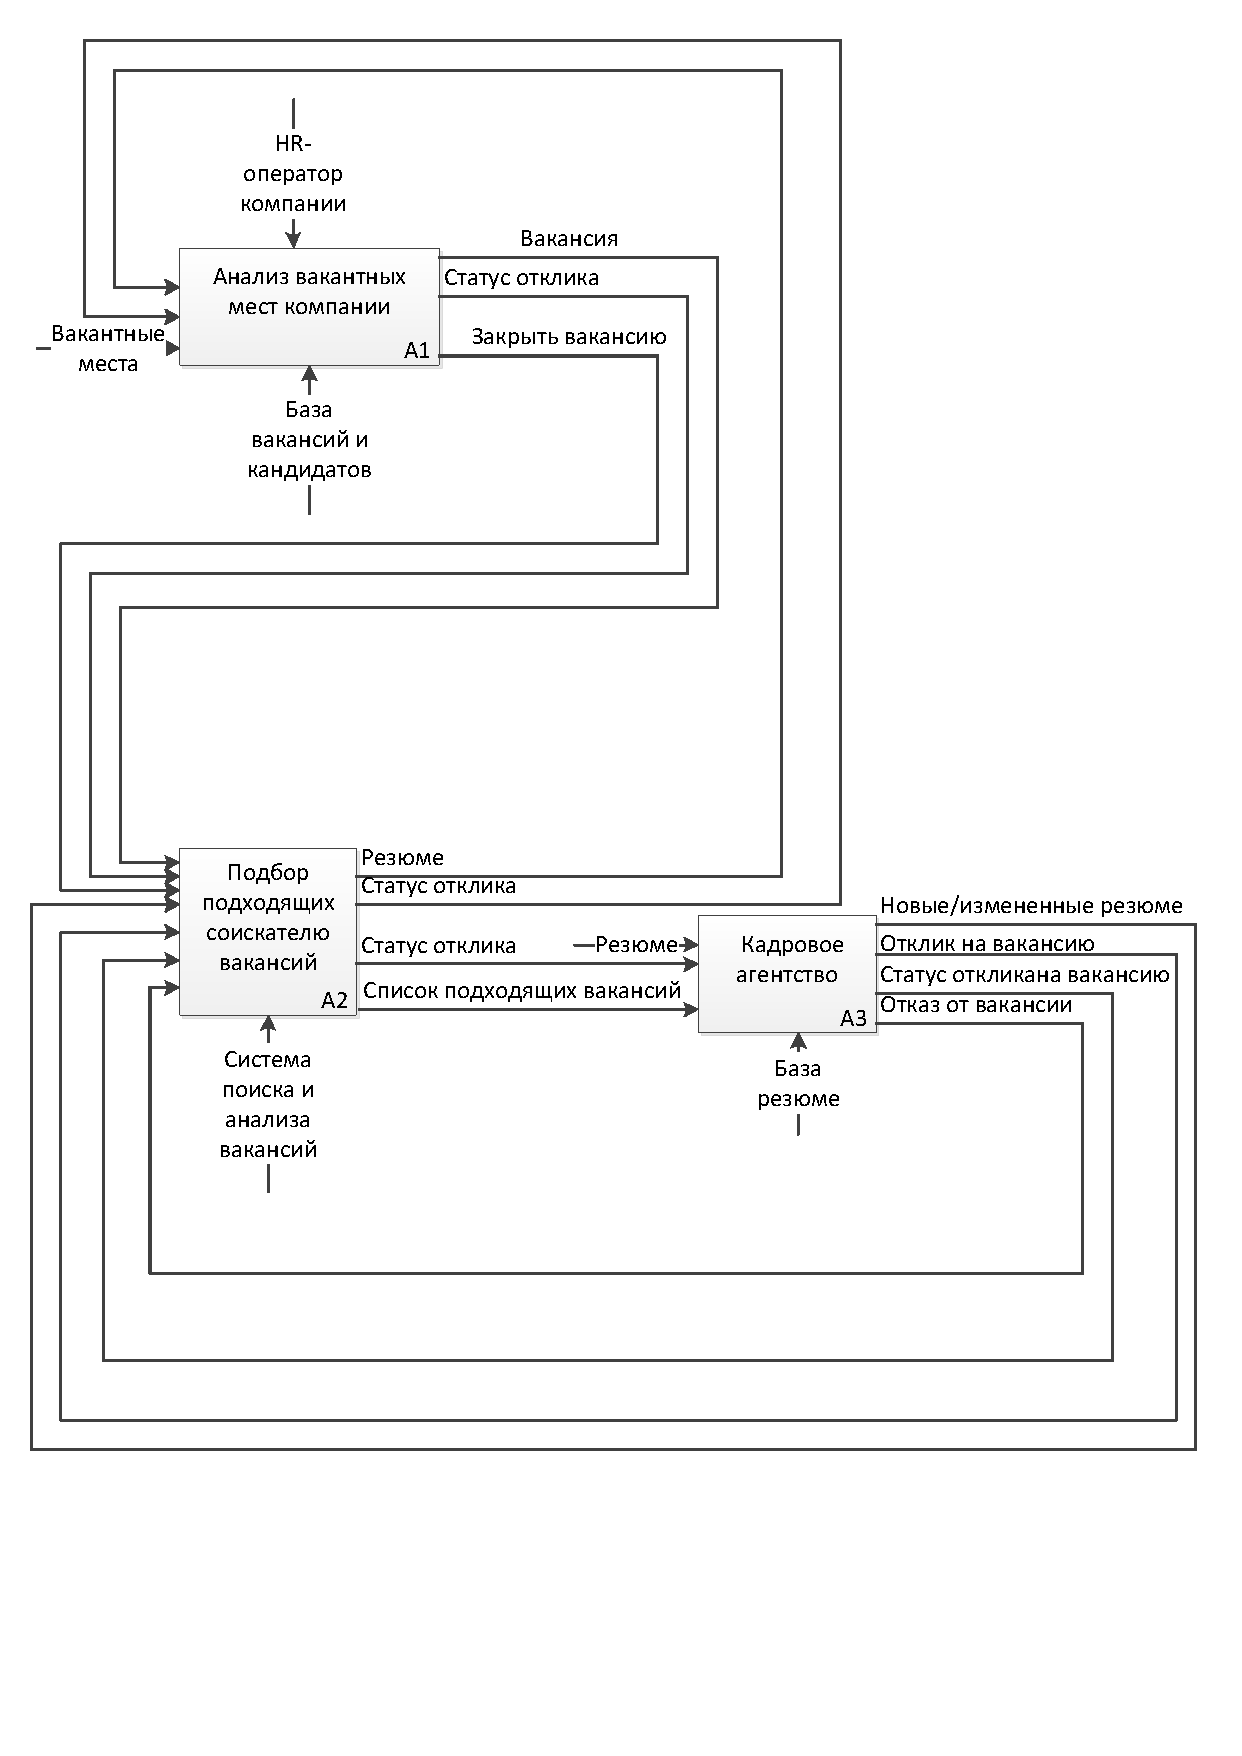
\includegraphics[width=\textwidth]{include/idef0.pdf}
\caption{Схема предметной области}
\label{fig:idef0}
\end{figure}

\section{Описание системы}
Разрабатываемая РСОИ состоит из трех типов узлов:
\begin{enumerate}
\item кадрового агентства;
\item отраслевой организации;
\item компании-нанимателя;
\end{enumerate} 

Рассмотрим функционирование каждого узла.
\begin{enumerate}[1.]
\item Кадровое агентство предоставляет соискателям графический интерфейс для создания резюме и обеспечивает удобное взаимодействие с предлагаемыми вакансиями от компаний-нанимателей.
\item Отраслевая организация принимает заявки от узлов компаний-нанимателей и кадровых агентств и обеспечивает логику обработки поступающих данных. А главное, на нем автоматически для каждой поступившей вакансии запускается поиск подходящих кандидатов, а для каждого нового кандидата список возможных вакансий.
\item Узел компании-нанимателя предоставляет интерфейс для оператора HR-отдела, позволяющий создавать заявки о вакантных местах с указанием критериев к соискателям, а также отклонять или принимать отклики от возможных кандидатов.
\end{enumerate}

\section{Сценарии функционирования системы со стороны соискателя}
\subsubsection{Регистрация соискателя}
Регистрация позволяет завести резюме.
Для регистрации надо:
\begin{enumerate}
\item указать имя, фамилию, отчество и дату рождения (зарегистрироваться может только совершеннолетний соискатель)
\item указать адрес электронной почты. Надо указывать реальный адрес, по которому в дальнейшем с вами свяжутся работодатели.
\item указать пароль
\end{enumerate}
\subsection{Аутентификация соискателя}
Аутентификация возможна только для зарегистрированных пользователей. Аутентификация позволяет просматривать и редактировать данные о себе, а также взаимодействовать с предлагаемыми вакансиями.
Для аутентификации надо:
\begin{enumerate}
\item указать адрес электронной почты в качестве логина
\item указать пароль
\end{enumerate}
\subsection{Заполнение данных об образовании}
Данные о вузе и специальности служат одним из критериев отбора, поэтому важно заполнить информацию об уже полученном (или получаемым в данный момент) образовании. Также немаловажную роль играет знание соискателем языков.
Заполнение данных о себе:
\begin{enumerate}
\item пройдите процедуру аутентификации соискателя
\item чтобы приступить к заполнению данных, выберите вкладку "Редактировать данные о себе" 
\item для того чтобы добавить образование, нажмите на кнопку "Добавить университет"
\item выберите название университета
\item выберите тип обучения
\item напишите свою специальность
\item укажите дату окончания университета
\item для того чтобы удалить данные об этом образовании, нажмите "Удалить университет"
\item для того чтобы добавить данные о знании языка, нажмите кнопку "Добавить язык"
\item выберите язык из списка
\item выберите уровень владения языком
\item чтобы данные были сохранены в базе, нажмите кнопку "Сохранить"
\end{enumerate}
\subsection{Создание резюме/поиск работы}
Только после создания резюме, данные соискателя будут отправлены на узел отраслевой организации. В резюме указываются не только возможности кандидата, но и его пожелания к будущей должности. От выбора сферы деятельности, зависит то, в какую отраслевую организацию будет отправлено резюме.
Чтобы создать/изменить резюме:
\begin{enumerate}
\item пройдите процедуру аутентификации соискателя
\item чтобы приступить к заполнению данных, выберите вкладку "Резюме" 
\item для добавления нового резюме, нажмите кнопку "Добавить резюме"
\item выберите интересующую отрасль из списка
\item выберите график работы
\item выберите график командировок
\item введите максимальную и минимальную заработную плату, которую вы ожидаете
\item введите желаемую должность
\item заполните данные о работе в аналогичной сфере - навыки, опыт работы (в годах)
\item Для внесения изменений в базу, а также отправку данных отраслевым агентствам, нажмите "Сохранить/Обновить резюме" 
\end{enumerate}
\subsection{Отказ от рассмотрения вакансии на любом этапе оценки кандидата}
Соискатель имеет полное право отказаться от вакансии, если она для него больше не актуальна, также он может отказаться даже от просмотра ее в списке возможных предложений, в таком случае, компания еще не знает о наличие кандидата и соотвественно, ей не отсылается сообщение с отказом.
\begin{enumerate}
\item пройдите процедуру аутентификации соискателя
\item если нет резюме или оно уже устарело, создайте/измените его на вкладке "Резюме"
\item выберите вкладку "Показать вакансии"
\item нажмите кнопку "Отказать" под выбранным предложением вакансии. 
\end{enumerate}
\subsection{Переход кандидата к очередному этапу отбора}
\begin{enumerate}
\item пройдите процедуру аутентификации соискателя
\item если нет резюме или оно уже устарело, создайте/измените его на вкладке "Резюме"
\item выберите вкладку "Показать вакансии"
\item нажмите кнопку "Принять" под выбранным предложением вакансии
\end{enumerate}

\section{Сценарии функционирования системы со стороны оператора HR-отдела компании}
\subsection{Создание вакансии/поиск кандидатов}
\begin{enumerate}
\item выберите вкладку "Редактор вакансий"
\item введите название позиции
\item введите требования к кандидату в поле "О позиции"
\item выберите отрасль
\item выберите график работы
\item выберите график командировок
\item введите минимальную и максимальную зарплату, на которую может рассчитывать кандидат
\item введите ожидаемый минимальный опыт работы кандидата
\item для добавления требований к знаниям языков, нажмите кнопку "Добавить языковые требования к кандидату" и выберите язык и уровень владения языка
\item для удаления требований к знаниям языков, нажмите кнопку "Удалить язык"
\item для добавления требований к образованию кандидата, нажмите кнопку "Добавить ожидаемое от кандидата образование", выберите университет и введите специальность
\item для удаления требований к образованию кандидата, нажмите кнопку "Удалить образование"
\item чтобы сохранить введенные данные в базе и отправить данных отраслевым агентствам, нажмите "Сохранить позицию" 
\end{enumerate}
\subsection{Отказ от рассмотрения кандидата}
\begin{enumerate}
\item если нет сохраненных вакансий или они устарели, создайте или измените позицию
\item выберите вкладку "Возможные кандидаты"
\item выберите соответствующего кандидата
\item нажмите кнопку "Отказать"
\end{enumerate}
\subsection{Переход кандидата к очередному этапу отбора}
\begin{enumerate}
\item если нет сохраненных вакансий или они устарели, создайте или измените позицию
\item выберите вкладку "Возможные кандидаты"
\item выберите соответствующего кандидата
\item нажмите кнопку "Принять"
\end{enumerate}
\subsection{Закрытие вакансии}
\begin{enumerate}
\item выберите вкладку "Редактор вакансий"
\item для удаления вакансии, нажмите "Удалить позицию"
\end{enumerate}

Основной сценарий взаимодействия пользователя с системой представляет собой последовательность следующих действий:
\begin{enumerate}
\item пользователь заходит на веб-интерфейс системы управления заявками;
\item пользователь создает заявку, указав интересующие критерии отбора необходимого кандидата;
\item HR-агентства, обрабатывающие заявку, выполняют поиск резюме по известным им хранилищам, отбирают кандидатов и представляют их резюме пользователю
\item пользователь отбирает кандидатов и закрывает заявку
\end{enumerate}

\section{Требования к системе}
На основе анализа предметной области необходимо сформулировать требования как ко всей системе, так и к ее подсистемам.

\subsection{Высокоуровневые требования к системе}
\begin{enumerate}
\item Система должна поддерживать добавление новых узлов.
\item Система не должна выходить из строя при выходе из строя одной из подсистем.
\item Обмен информации в системе должен производиться исходя из предположения, что каналы связи небезопасны и ненадежны.
\item Система должна предусматривать восстановление в случае сбоя.
\end{enumerate}

\subsection{Требования к системе кадрового агентства}

\textbf{Функциональные требования}
\begin{enumerate}
\item Система должна предоставлять пользователю веб-интерфейс.
\item Система должна осуществлять регистрацию и аутентификацию уже зарегистрированных пользователей.
\item Система должна предоставлять пользователю возможность создания/редактирования данных о себе
\item Система должна предоставлять пользователю список подходящих вакантных мест, с возможностью отклика или отказа от них.
\item Система должна оповещать пользователя об изменении состояния отклика на вакансию.
\end{enumerate}

\subsection{Требования к системе компании-нанимателя}
\textbf{Функциональные требования}
\begin{enumerate}
\item Система должна предоставлять оператору веб-интерфейс.
\item Система должна предоставлять возможность для добавления, изменения и удаления данных о вакантных местах.
\item Система должна предоставлять список откликнувшихся кандидатов и инструменты для дальнейшего управления процессом отбора
\end{enumerate}

\subsection{Требования к системе отраслевые организации}
\textbf{Функциональные требования}
\begin{enumerate}
\item Система должна принимать данные о соискателях и о вакансиях, преобразуя их в список критериев
\item Система должна анализировать критерии резюме и подбирать список подходящих вакансий.
\end{enumerate}

\textbf{Вывод}

После анализа предметной области и протекающих  них процессов были выделены подсистемы распределенной системы и сформулированы требования к ним.


%%% Local Variables:
%%% mode: latex
%%% TeX-master: "rpz"
%%% End:

\chapter{Конструкторский раздел}
\label{cha:design}
В данном разделе описывается процесс проектирования субъектов разрабатываемой распределенной системы: кадрового агентства, отраслевой организации, компании-нанимателя, а также их взаимодействия.

\section{Структура разрабатываемой распределенной системы}
Разрабатываемая распределенная система состоит из субъектов трех видов:
\begin{enumerate}
\item кадрового агентства;
\item системы компании-нанимателя;
\item отраслевой организации;
\end{enumerate}

Структура системы представлена на рисунке ~\ref{fig:structure}. 

\begin{figure}[h!]
  \centering
  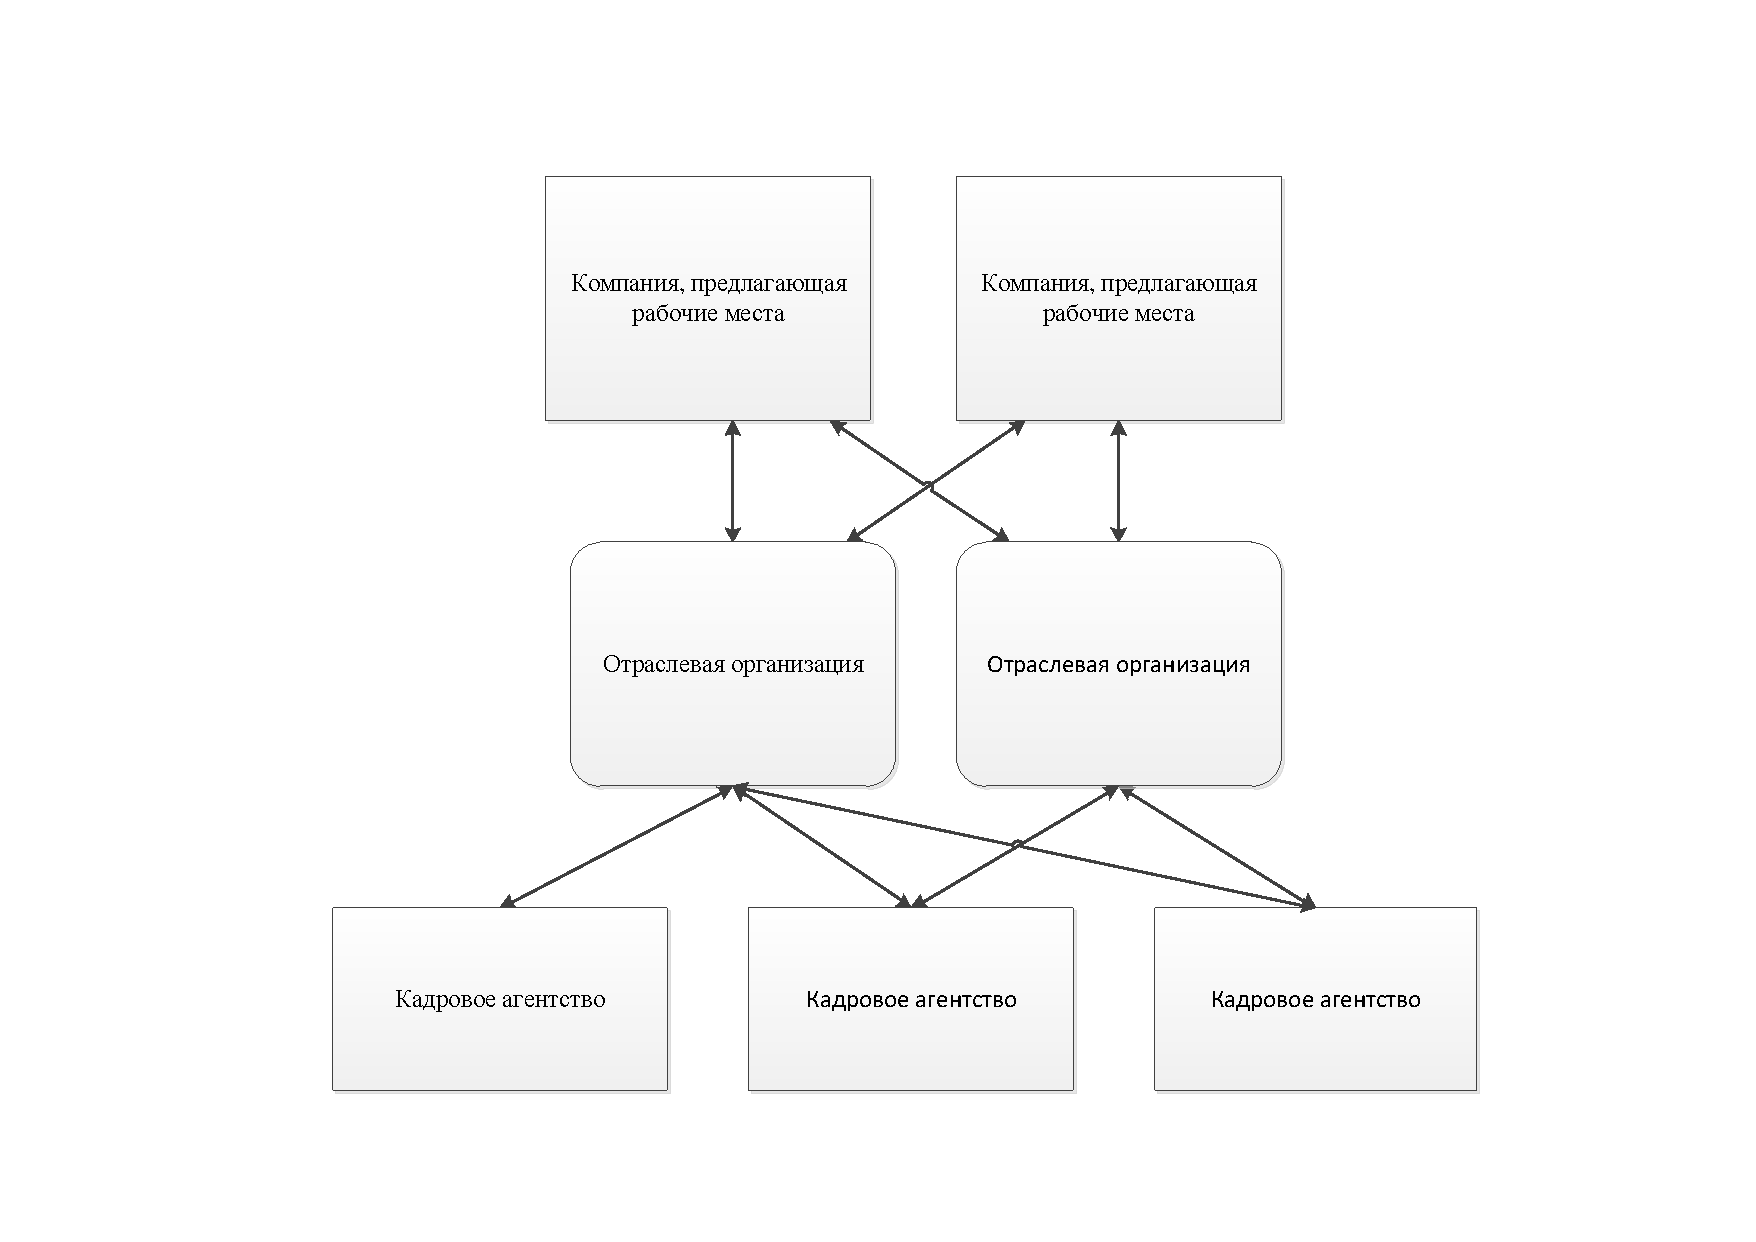
\includegraphics[width=\textwidth]{include/UML.pdf}
  \caption{Структура разрабатываемой распределенной системы}
  \label{fig:structure}
\end{figure}

\textbf{Система кадровое агентство} предоставляет пользователям графический интерфейс для создания и изменения резюме, а также для просмотра и взаимодействия с предлагаемыми вакансиями.

\textbf{Система компании-нанимателя} отвечает предоставляет оператору HR-отдела графический интерфейс для создания и редактирования вакансий, а также просмотра и обработки данных откликнувшихся кандидатов. 

\textbf{Система отраслевая организация} обрабатывает поступающие от компании-нанимателя и кадрового агентства заявки. Она выполняет поиск и отбор вакансий и кандидатов.


\section{Система кадрового агентства}
В данном разделе описывается структура и функционирование системы кадровое агентство. 

\subsection{Модель данных}
Данные системы кадрового агентства содержат следующие сущности, связь которых представлена на рисунке ~\ref{fig:data-model-empui}.

\begin{figure}[h!]
\centering
 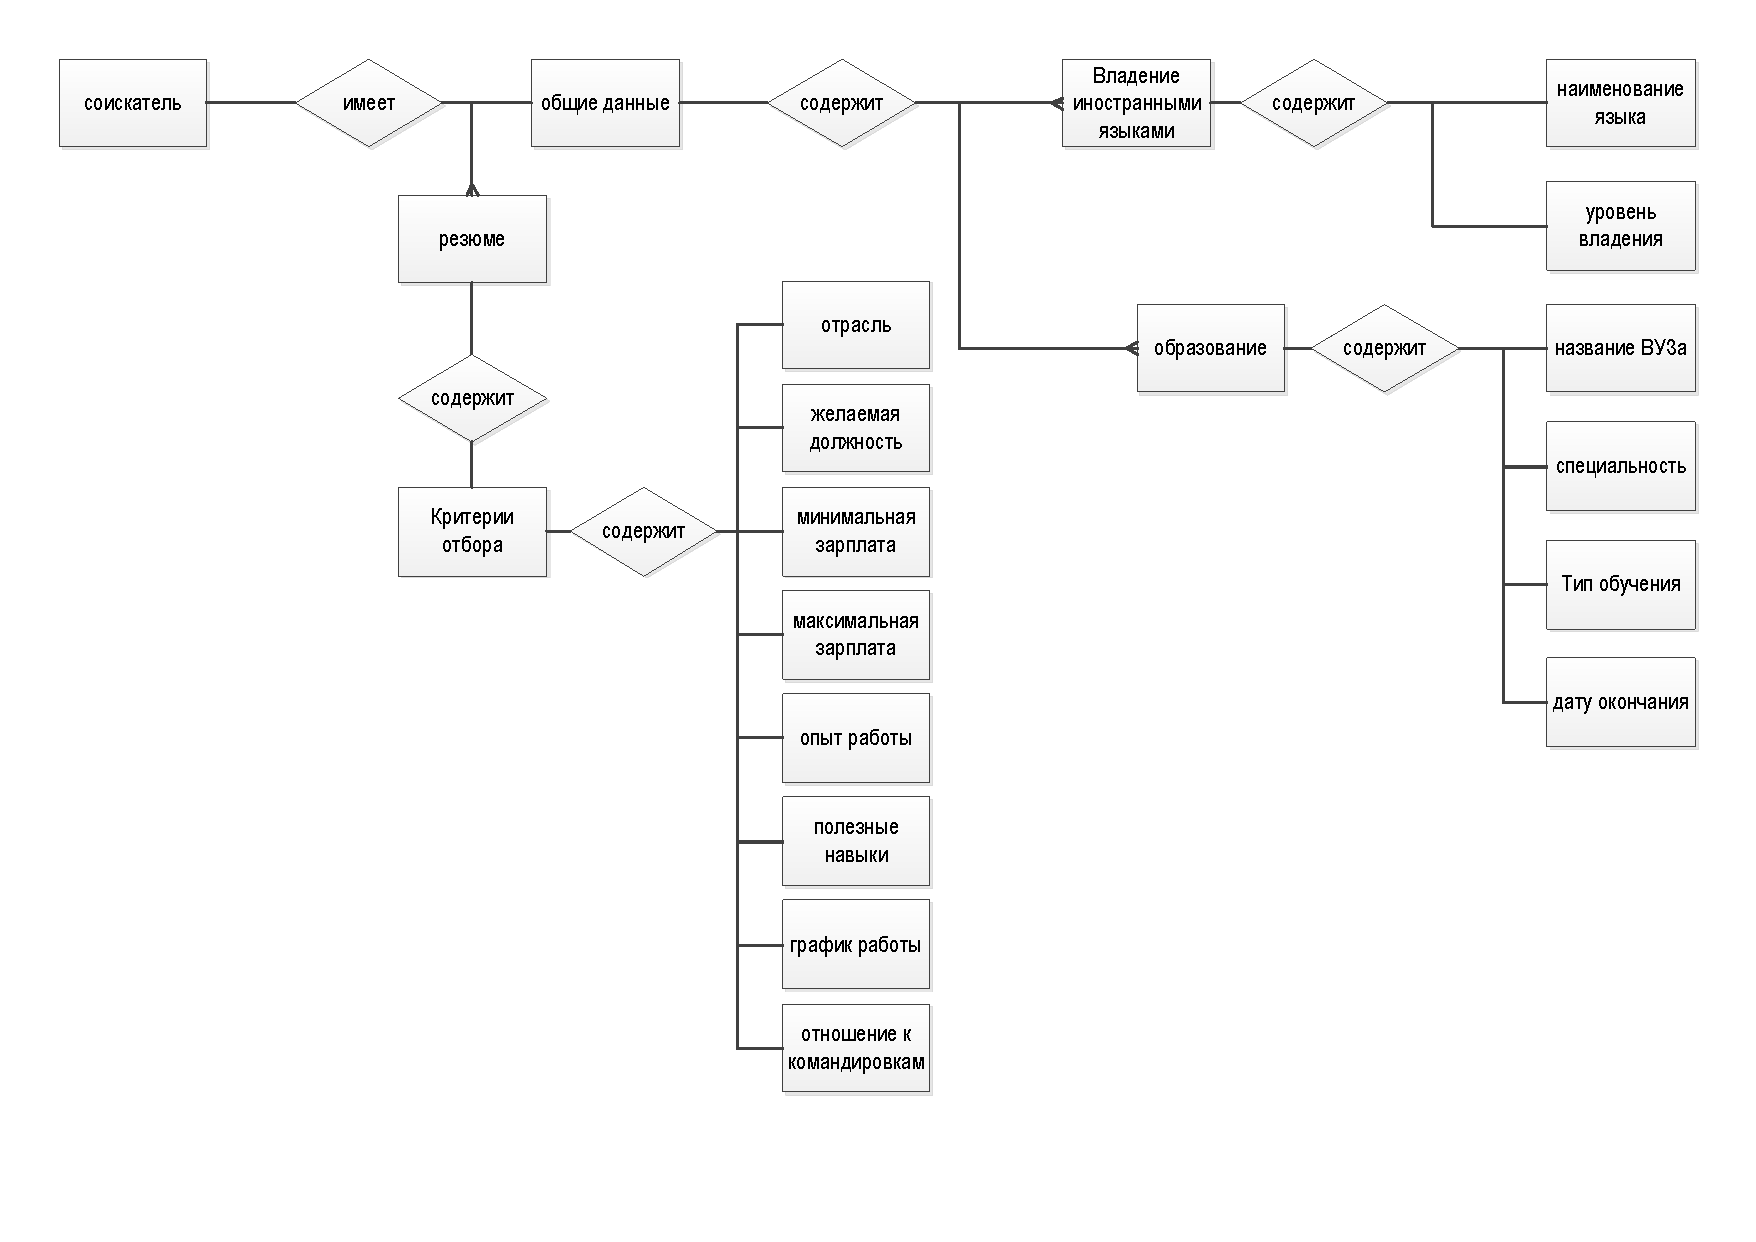
\includegraphics[width=1\textwidth]{include/data-model-cvcol.pdf}
\caption{ER-диаграмма системы кадрового агентства}
\label{fig:data-model-empui}
\end{figure}

\begin{enumerate}
\item Пользователи - содержит информацию о зарегистрированных пользователях системы: почтовый адрес и пароль, а так же ФИО, дата рождения, образование и прочие личные данные;
\item Заявки – содержит данные резюме. В них хранятся заголовок, идентификатор пользователя в данной системе, данные-критерии отбора;
\item Критерии графика работы, занятости, опыта работы, профессиональной области содержат информацию о доступных критериях поиска.
\end{enumerate}

\subsection{Обработка заявки в системе}
Жизненный цикл заявки включает в себя 7 состояний:
\begin{enumerate}
\item $>0$ - заявка ожидает отклика соискателя;
\item $=0$ - отказ в дальнейшем рассмотрении заявки;
\item $=-1$ - соискатель откликнулся на вакансию;
\item $=-2$ - соискателю предложили пройти собеседование.
\item $=-3$ - соискатель согласился пройти собеседование.
\item $=-4$ - соискателю сделали предложение о работе.
\item $=-5$ - соискатель готов приступить к работе.
\item $=-6$ - вакансия закрыта.
\end{enumerate}
Система кадрового агентства отражает состояние заявки, изменения которой вызывают действия пользователя или системы компании-нанимателя.

\section{Система компании-нанимателя}
В данном разделе описывается структура и функционирование системы компании-нанимателя. 

\subsection{Модель данных}
Данные системы компании-нанимателя содержат следующие сущности, связь которых представлена на рисунке ~\ref{fig:data-model-emp}.

\begin{figure}[h!]
\centering
 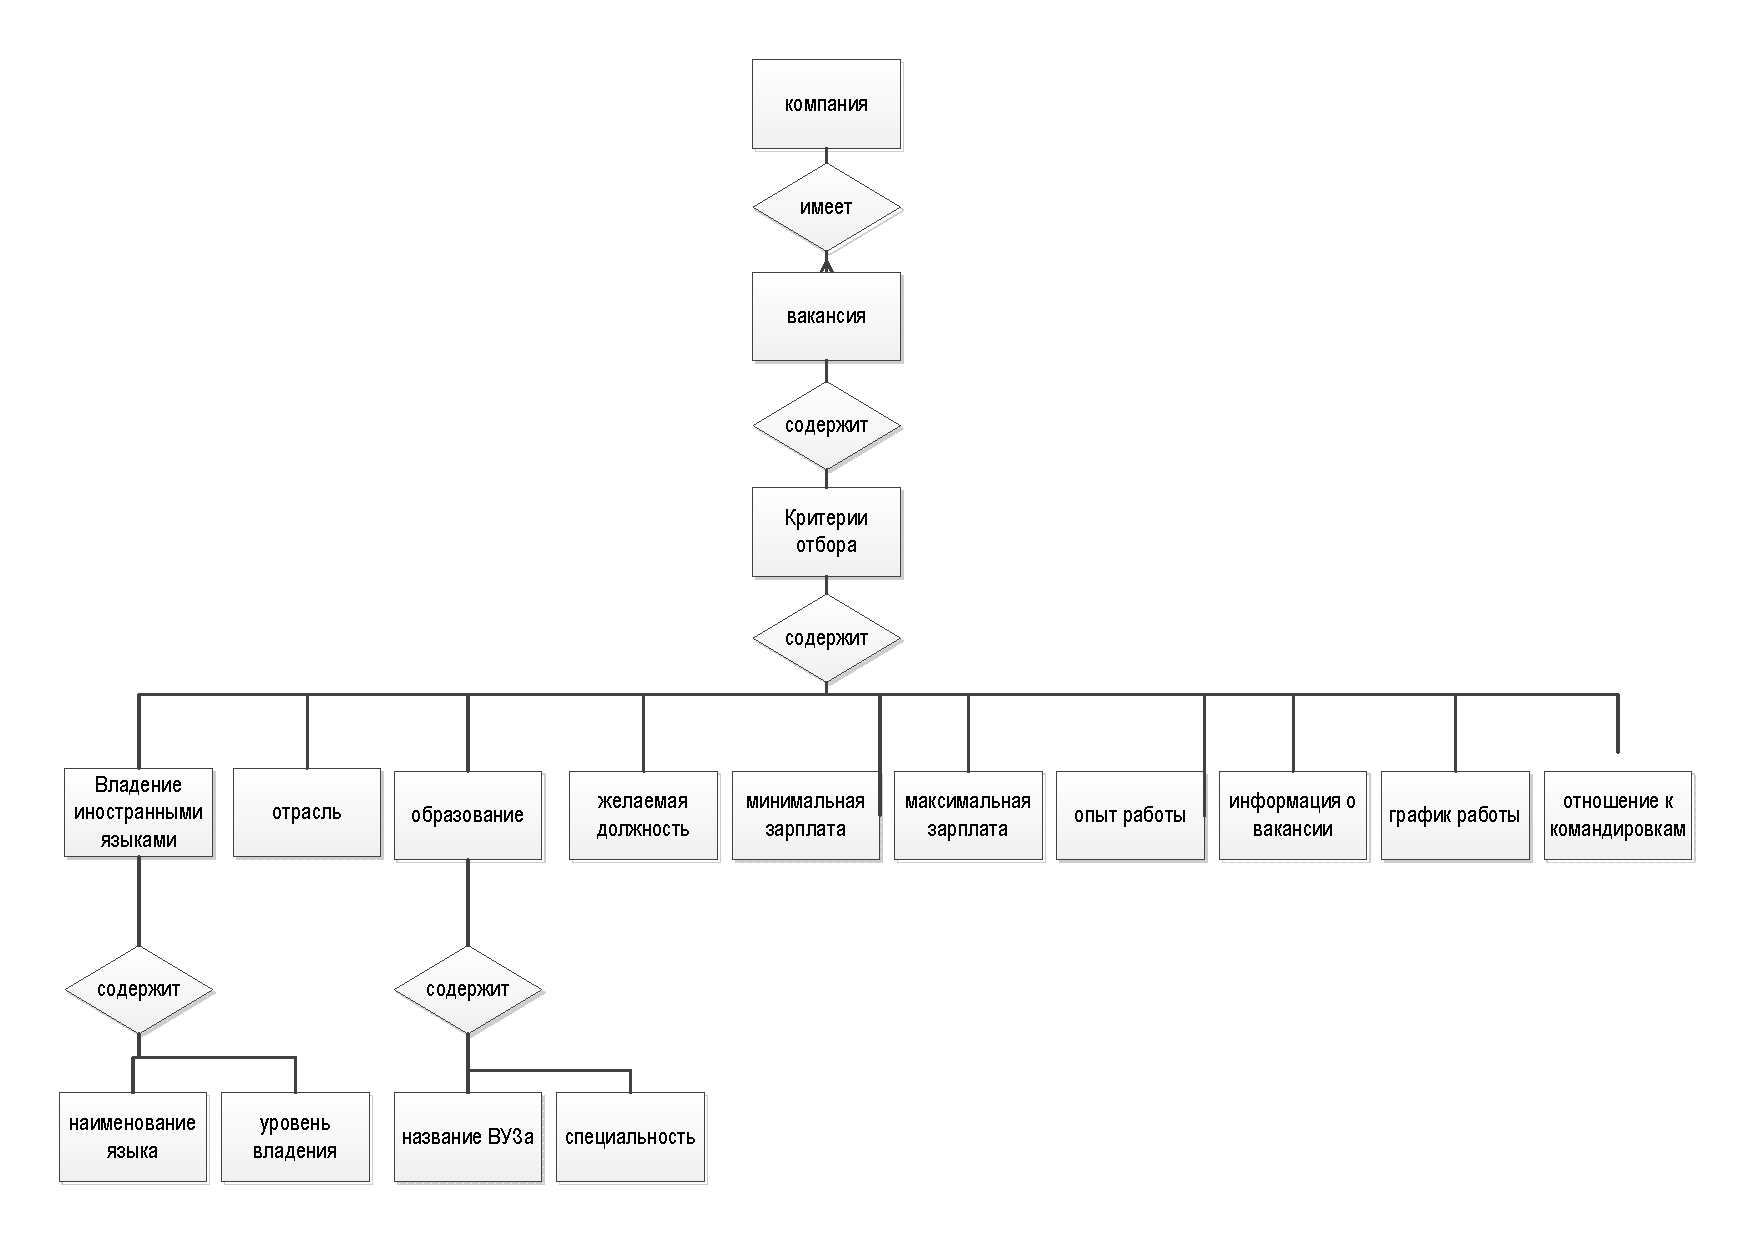
\includegraphics[width=\textwidth]{include/data-model-emp.pdf}
\caption{ER-диаграмма системы компании-нанимателя}
\label{fig:data-model-emp}
\end{figure}

\begin{enumerate}
\item Пользователи - содержит информацию о зарегистрированных пользователях системы: почтовый адрес и пароль, а так же ФИО, дата рождения, образование и прочие личные данные;
\item Заявки – содержит данные резюме. В них хранятся заголовок, идентификатор пользователя в данной системе, данные-критерии отбора;
\item Критерии графика работы, занятости, опыта работы, профессиональной области содержат информацию о доступных критериях поиска.
\end{enumerate}

\subsection{Обработка заявки в системе}
Жизненный цикл заявки включает в себя 6 состояний:
\begin{enumerate}
\item $=0$ - отказ в дальнейшем рассмотрении заявки;
\item $=-1$ - соискатель откликнулся на вакансию;
\item $=-2$ - соискателю предложили пройти собеседование.
\item $=-3$ - соискатель согласился пройти собеседование.
\item $=-4$ - соискателю сделали предложение о работе.
\item $=-5$ - соискатель готов приступить к работе.
\item $=-6$ - вакансия закрыта.
\end{enumerate}
Система компании-нанимателя отражает состояние заявки, изменения которой вызывают действия оператора HR-агентства или соискателей.

\section{Система отраслевых организаций}
В данном разделе описывается структура и функционирование системы отраслевой организации.

Отраслевая организация выполняет роль промежуточного звена - содержа в себе одновременно и запросы соискателей, и критерии работодателей. Также она обладает автоматической системой подбора персонала, результатом такой обработки является связь многие ко многим между идентификаторами вакансий и идентификаторами соискателей.


\section{Протокол взаимодействия систем}
Субъекты РСОИ должны взаимодействовать по формализованному протоколу взаимодействия. В этом параграфе описывается последовательность и формат передаваемых сообщений.

\subsection{Последовательность передаваемых сообщений}
Для реализации взаимодействия субъектов распределенной системы друг с другом используется как синхронный, так и асинхронный подход. Взаимодействие систем проиллюстрировано на диаграмме последовательностей на рисунке ~\ref{fig:state-diag-hr}.

\begin{figure}[h!]
\centering
 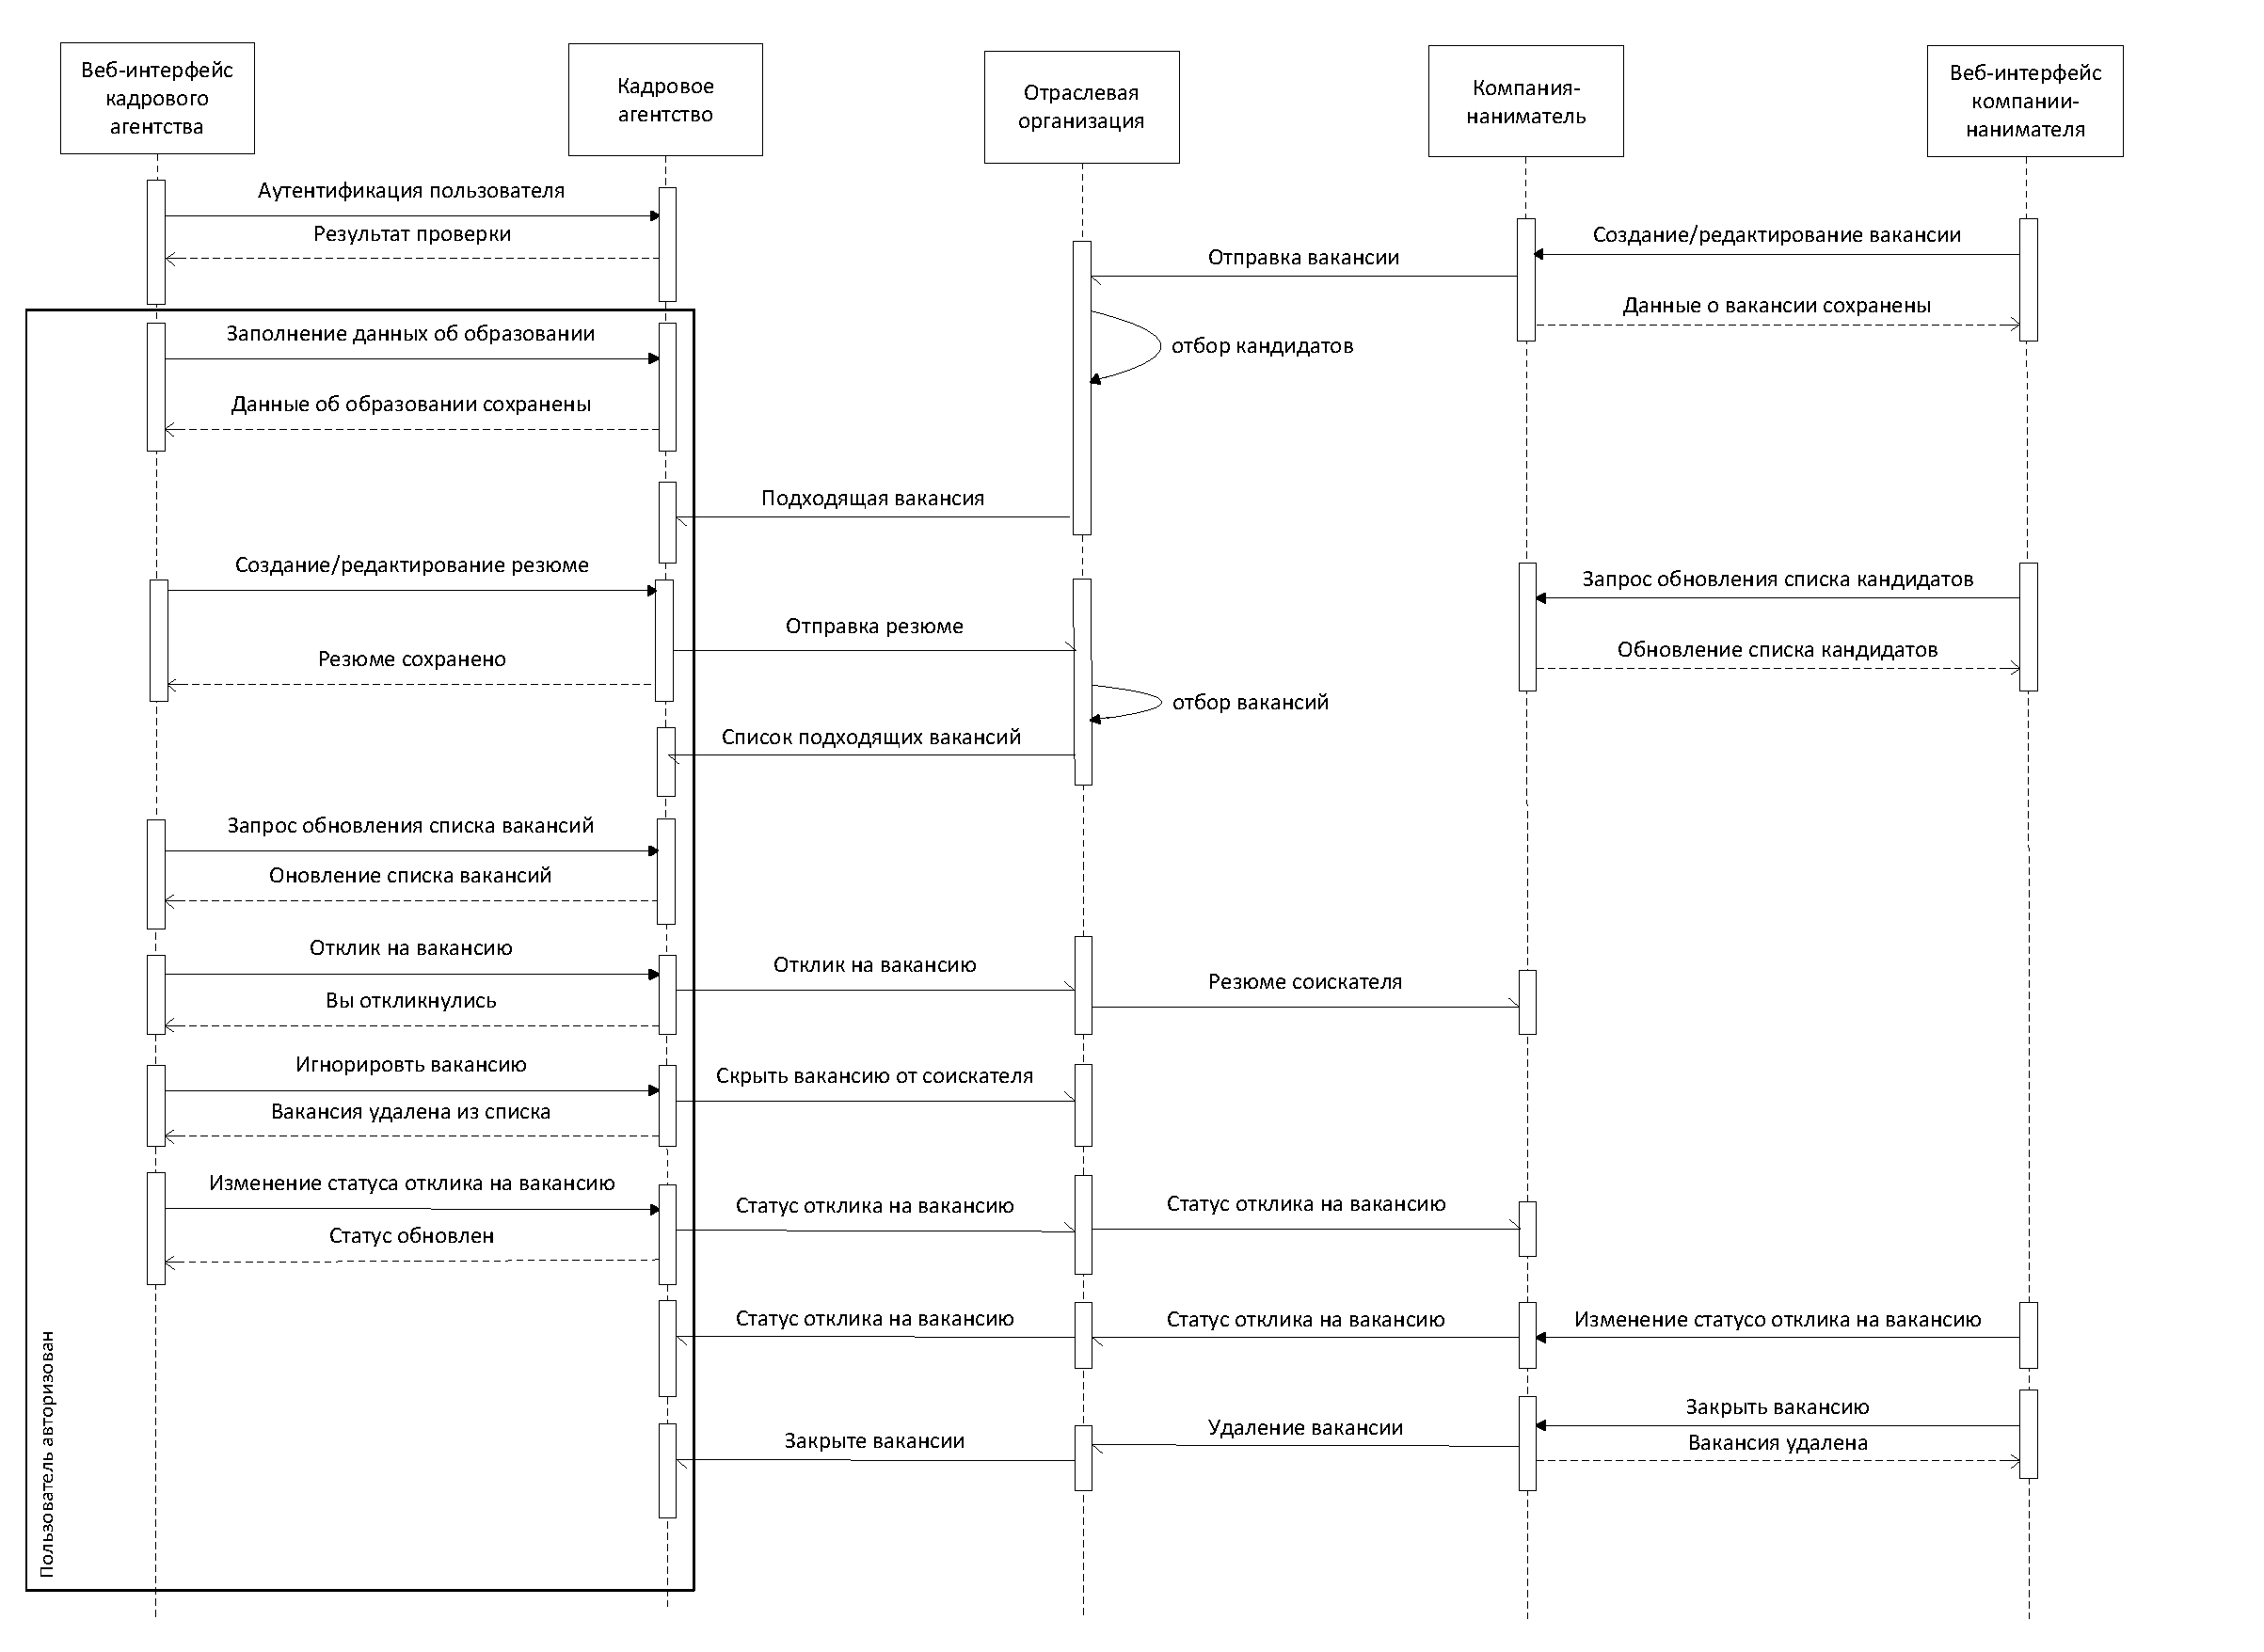
\includegraphics[width=1.1\textwidth]{include/activity-diag2.pdf}
\caption{Последовательность взаимодействия систем при регистрации вакансий и резюме}
\label{fig:state-diag-hr}
\end{figure}

Процесс поиска вакансии начинается с регистрации пользователя на сайте кадрового агентства. После заполнения всех необходимых данных и аутентификации, пользователь получает доступ к заполнению информации об образовании, знании иностранных языков, а также к созданию резюме.
После введения всех необходимых данных, а так же заполнении своих ожиданий, навыков, опыта и прочих важных в отборе критериев, пользователь может сохранить резюме. 
Сохранение происходит в базе самого кадрового агентства, затем из всех данных о пользователе формируется заявка для отправки в ту отраслевую организацию, специализация которой указана в резюме. 

На узле отраслевой организации поступившая заявка сохраняется, производится поиск всех вакансий, чей критерий сходства не меньше $0.4$.

Для этого поочередно сравниваются данные пользователя и указанные требования. 
Для увеличения коэффициента сходства необходимо:
\begin{enumerate}
\item опыт работы соискателя $\geqslant$  указанного в вакансии
\item ожидаемая минимальная заработная плата $\leqslant$ максимальная заработная плата, предлагаемая компанией
\item если соискатель готов к любым командировкам, то неважно, что указано в этом пункте в вакансии, иначе же отношение к командировкам должно совпадать
\item соискатель может быть готов работать полный день, либо график работы должен совпадать с указанным в вакансии
\item если список иностранных языков в вакансии включает в себя языки известные соискателю, то коэффициент увеличивается, если пользователь указал все языки, перечисленные в вакансии, коэффициент увеличивается еще раз
\item если список предпочитаем университетов в вакансии включает в себя университеты соискателя, то коэффициент увеличивается, если в список университетов, в которых учился или учится соискатель есть все перечисленные в вакансии, коэффициент увеличивается еще раз
\item особым образом идет сравнение названия вакансии и поста, на который претендует соискатель. Это две строки, лаконично описывающие должность, необязательно идентичных. Для сравнения подсчитывается количество слов совпавших в обоих строчках, после чего это количество делится на количество слов в строке, описывающей пост, на который претендует соискатель. Если частное больше $0.4$, то коэффициент сходства увеличивается на один
\item аналогичным способом идет сравнение специальности соискателя и специальности указанной в вакансии
\item полученный коэффициент сходства делится на максимально возможный и результат возвращается в таблицу отношений вакансия - соискатель
\end{enumerate} 

После окончания поиска, пользователю отсылается список подходящих вакансий.
Узел кадрового агентства имеет веб-интерфейс и позволяет просматривать поступившие уведомления содержимым вакансий, а также взаимодействовать с ними.
Вначале вакансия имеет статус "Ожидание подтверждения готовности рассмотреть вакансию". После этого есть возможность сразу отказаться от дальнейшего рассмотрения этой вакансии, тогда, эта вакансия будет удалена из базу кадрового агентства, а также отмечена на узле отраслевой организации, в таблице отношений вакансия-соискатель как игнорируемая (статус 0). Если же соискатель ответит отказом уже после отклика, то после отраслевой организации, заявка-отказ отправится на узел соответствующей компании.
Если же откликнуться, то строка статуса тут же сообщит об этом. Отраслевой организации будет отправлен идентификатор пользователя, идентификатор позиции, ФИО и полезные навыки (в базе самой отраслевой организации не хранятся имена пользователей, а также их навыки). 
На узле отраслевой организации осуществляется сбор информации по этому пользователю, добавляются вновь пришедшие данные и полученное сообщение отправляется дальше - на узел кадрового агентства.

Кадровое агентство также имеет визуальный интерфейс.
Информация соискателя отобразится в списке, можно отклонить претендента и тогда на узле отраслевой организации, в таблице отношений вакансия-соискатель соответствующая строка будет установлена как игнорируемая (статус 0), а у претендента в строке состояния отразится сообщение об отказе. 
Если нажать кнопку принять, тогда заявка перейдет в следующее состояние. И так вплоть до предложения о работе и принятия его соискателем.

При регистрации новой вакансии, данные о ней сохраняются в базе, а критерии отправляются в соответствующую отраслевую организацию. Там происходит аналогичный поиск подходящих резюме и найденным претендентам рассылается предложение с информацией о вакансии.



Для реализации взаимодействия веб-интерфейсов и компании-нанимателя или же кадрового агентства используется синхронный подход. После запуска процедуры создания заявки системы выполняют ее сохранение в базе и возвращают в веб-интерфейс сообщение об успехе или неудачи выполнения задачи. В случае успешного создания заявок системы выполняют асинхронное отправление заявок по зарегистрированным в них отраслевым организациям.

По получению новой заявки в системе отраслевые организации обрабатывают ее, подыскивая подходящие вакансии или кандидатов. После чего отправляет отобранные вакансии соответствующим кадровым агентствам, с указанием идентификаторов соискателей.

Получив ответ от отраслевых организаций, компания-наниматель и кадровое агентство обновляют списки вакансий, соискателей, передавая изменения в веб-интерфейс.

В любой момент может быть инициировано закрытие заявки.


\subsection{Содержание передаваемых сообщений}
В процессе функционирования информационные системы, являющиеся подсистемами разрабатываемой РСОИ, взаимодействуют между собой, используя синхронную и асинхронную модель передачи сообщений. Для реализации этого взаимодействия необходимо определить данные, передаваемые в этих сообщениях.

В таблице ~\ref{tab:tab-messages} рассмотрены передаваемые между системами сообщения и информация, содержащаяся в них.
\begin{longtable}[ht]{|p{1,5cm}|p{3cm}|p{3cm}|p{3cm}|p{4,5cm}|}
\caption{Содержание сообщений, передаваемых между подсистемами РСОИ}\label{tab:tab-messages} \\
\hline
Тип & Название & Система- отправитель  & Система- получатель & Передаваемые данные \\
\hline\hline\endfirsthead
\caption{Содержание сообщений, передаваемых между подсистемами РСОИ (продолжение)} \\
\hline
Тип & Название & Система- отправитель  & Система- получатель & Передаваемые данные \\
\hline\hline\endhead
\hline
\multicolumn{4}{c}{\textit{Продолжение на следующей странице}}
\endfoot
\endlastfoot
Запрос (синхр.)	& Регистрация пользователя	& Веб-интерфейс кадрового агентства 	& Кадровое агентство	& email и пароль\\
\hline
Ответ	& Регистрация пользователя	& Кадровое агентство & Веб-интерфейс кадрового агентства	& Результат регистрации пользователя\\
\hline
Запрос (синхр.)	& Аутентификация пользователя	& Веб-интерфейс кадрового агентства 	& Кадровое агентство	& email и пароль\\
\hline
Ответ	& Аутентификация пользователя	& Кадровое агентство & Веб-интерфейс кадрового агентства	& Результат аутентификации пользователя\\
\hline
Запрос (синхр.)	& Запрос информации о образовании пользователя	& Веб-интерфейс кадрового агентства 	& Кадровое агентство	& Идентификатор пользователя\\
\hline
Ответ	& Запрос информации о образовании пользователя	& Кадровое агентство & Веб-интерфейс кадрового агентства	& Информация об образовании и знании иностранных языков\\
\hline
Запрос (синхр.)	& Список резюме пользователя	& Веб-интерфейс кадрового агентства 	& Кадровое агентство	& идентификатор пользователя\\
\hline
Ответ	& Список резюме пользователя	& Кадровое агентство & Веб-интерфейс кадрового агентства	& Список резюме\\
\hline
Запрос (синхр.)	& Список вакансий для пользователя	& Веб-интерфейс кадрового агентства 	& Кадровое агентство	& идентификатор пользователя\\
\hline
Ответ	& Список вакансий для пользователя	& Кадровое агентство & Веб-интерфейс кадрового агентства	& Список вакансий для пользователя\\
\hline
Запрос (синхр.)	& Сохранение данных об образовании & Веб-интерфейс кадрового агентства 	& Кадровое агентство	& Данные об образовании\\
\hline
Ответ	& Сохранение данных об образовании	& Кадровое агентство & Веб-интерфейс кадрового агентства	& Результат сохранения данных об образовании\\
\hline
Запрос (синхр.)	& Сохранение резюме & Веб-интерфейс кадрового агентства 	& Кадровое агентство	& Данные резюме\\
\hline
Ответ	& Сохранение данных резюме	& Кадровое агентство & Веб-интерфейс кадрового агентства	& Результат сохранения резюме\\
\hline
Запрос (синхр.)	& Изменение статуса вакансии & Веб-интерфейс кадрового агентства 	& Кадровое агентство	& Идентификатор вакансии, новый статус\\
\hline
Ответ	& Изменение статуса вакансии	& Кадровое агентство & Веб-интерфейс кадрового агентства	& Результат сохранения нового статуса\\
\hline
Запрос (асинхр.)	& Открытие/изменение резюме & Кадровое агентство & Отраслевая организация	& Данные резюме и образования, идентификатор пользователя\\
\hline
Ответ	& Открытие/изменение резюме & Отраслевая организация & Кадровое агентство	& Отобранные вакансии, идентификатор пользователя\\
\hline
Запрос (асинхр.)	& Отклик на вакансию & Кадровое агентство & Отраслевая организация	& Данные резюме и образования, идентификатор пользователя, текущий статус отклика\\
\hline
Ответ	& Отклик на вакансию  & Отраслевая организация & Компания- наниматель	& Список откликнувшихся пользователей\\
\hline
Запрос (асинхр.)	& Игнорировать вакансию & Кадровое агентство & Отраслевая организация	& Данные резюме и образования, идентификатор пользователя, статус - игнорирование вакансии\\
\hline
Запрос (асинхр.)	& Отказ от вакансии & Кадровое агентство & Отраслевая организация	& Данные резюме и образования, идентификатор пользователя, текущий статус - отказ\\
\hline
Ответ	& Отказ от вакансии  & Отраслевая организация & Компания- наниматель & Информация о резюме, статус - отказ\\
\hline
Запрос (асинхр.)	& Подтвердить переход к следующему этапу рассмотрения вакансии & Кадровое агентство & Отраслевая организация	& Данные резюме и образования, идентификатор пользователя, текущий статус\\
\hline
Ответ	& Подтвердить переход к следующему этапу рассмотрения вакансии  & Отраслевая организация & Компания- наниматель & Информация о резюме, статус\\
\hline
Запрос (асинхр.)	& Отправка резюме	& Отраслевая организация	& Компания- наниматель	& Данные резюме\\
\hline
Запрос (асинхр.)	& Открытие вакансии & Компания- наниматель & Отраслевая организация	& Данные вакансии\\
\hline
Ответ	& Открытие вакансии & Отраслевая организация & Кадровое агентство	& Данные вакансии, каждому из отобранных пользователей\\
\hline
Запрос (асинхр.)	& Закрытие вакансии & Компания- наниматель & Отраслевая организация	& Идентификатор вакансии\\
\hline
Ответ	& Закрытие вакансии & Отраслевая организация & Кадровое агентство	& Сообщение о закрытие вакансии, каждому из подписанных пользователей\\
\hline
Запрос (синхр.)	& Список резюме откликнувшихся пользователей	& Веб-интерфейс компании-нанимателя 	& Компания-наниматель	& -\\
\hline
Ответ	& Список резюме откликнувшихся пользователей	& Компания-наниматель & Веб-интерфейс компании-нанимателя	& Список резюме и названия вакансий\\
\hline
Запрос (синхр.)	& Список доступных вакансий	& Веб-интерфейс компании-нанимателя 	& Компания-наниматель	& -\\
\hline
Ответ	& Список доступных вакансий	& Компания-наниматель & Веб-интерфейс компании-нанимателя	&  Список доступных вакансий\\
\hline
Запрос (синхр.)	& Сохранение данных о вакансии & Веб-интерфейс компании-нанимателя 	& Компания-наниматель	& Данные о вакансии \\
\hline
Ответ	& Сохранение данных о вакансии	& Компания-наниматель & Веб-интерфейс компании-нанимателя	& Результат сохранения данных о вакансии \\
\hline
Запрос (асинхр.)	& Отказ от рассмотрения резюме & Компания-наниматель & Отраслевая организация	& Идентификатор резюме, идентификатор вакансии, текущий статус - отказ\\
\hline
Ответ	& Отказ от рассмотрения резюме  & Отраслевая организация & Кадровое агентство & Идентификатор резюме, идентификатор вакансии, текущий статус - отказ\\
\hline
Запрос (асинхр.)	& Подтвердить переход к следующему этапу рассмотрения резюме & Компания- наниматель & Отраслевая организация	& Идентификатор резюме, идентификатор вакансии, текущий статус\\
\hline
Ответ	& Подтвердить переход к следующему этапу рассмотрения вакансии  & Отраслевая организация & Кадровое агентство & Идентификатор резюме, идентификатор вакансии, статус\\
\hline

\end{longtable}






























\chapter{Технологический раздел}
\label{cha:impl}
В данном разделе описываются технические средства, используемые при проектировании распределенной системы обработки информации. Также приведены результаты разработки системы.

\section{Среда разработки и язык программирования}
Разработка РСОИ осуществлялась на языке Python.
Выбор данного языка программирования обусловлен платформонезависимостью, большим количеством своих и сторонних библиотек, а также наличием его в списке рекомендуемых кафедрой.

В качестве дополнительных иблиотек использовались:
\begin{enumerate}
\item CherryPy — объектно-ориентированный веб-фреймворк, написанный на языке программирования Python. Спроектирован для быстрой разработки веб-приложений для сети Интернет. Представляет собой надстройку над HTTP-протоколом, но остаётся на низком уровне и не выходит за рамки требований RFC 2616.
\item SQLAlchemy - программная библиотека на языке Python для работы с реляционными СУБД с применением технологии ORM. 
\end{enumerate}

В качестве СУБД использовался sqlite - легковесная встраиваемая реляционная база данных, модуль которой встроен в Python по-умолчанию.

\section{Выбор протоколов взаимодействия}
\subsection{Протокол асинхронного взаимодействия}
В качестве протокола асинхронного взаимодействия были выбраны протоколы SMTP/POP3, так как они есть в списке рекомендуемых кафедрой протоколов для выполнения курсового проектирования.

\subsection{Протокол синхронного взаимодействия}
В качестве протокола синхронного взаимодействия был использован протокол HTTP.

\section{Диаграммы классов}
\subsection{Диаграмма классов системы кадрового агентства}
Диаграмма классов представлена на рисунке ~\ref{fig:Visio-hh-uml}.

\begin{figure}[ht!]
\centering
 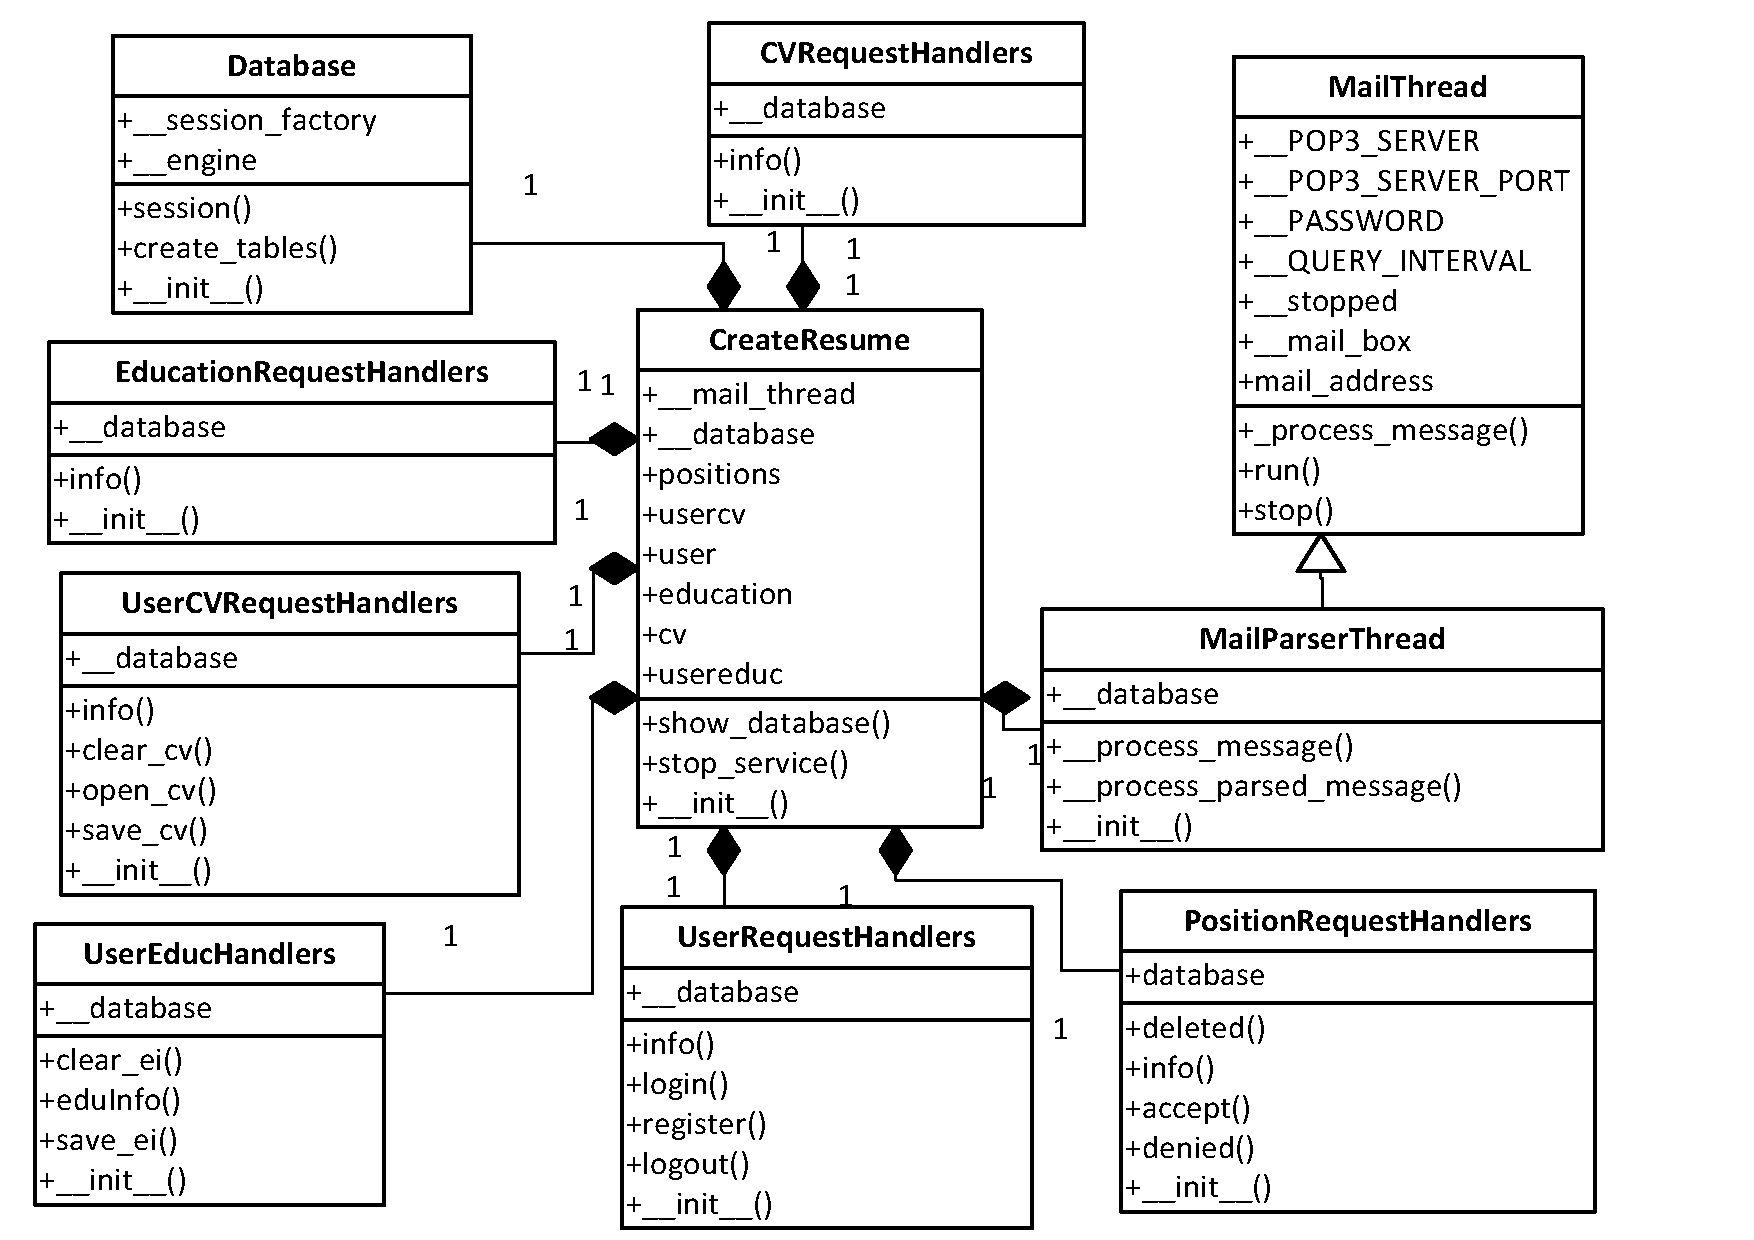
\includegraphics[width=\textwidth]{include/Visio-hh-uml.pdf}
\caption{Диаграмма классов системы кадрового агентства}
\label{fig:Visio-hh-uml}
\end{figure}

Ниже приведена спецификация классов системы кадрового агентства.

\textbf{Спецификация классов системы кадрового агентства}
\begin{enumerate}
\item EducationRequestHandlers – класс, выполняющий отправку списка возможных параметров образования в веб-интерфейс.
	\begin{enumerate}
	\item info – метод возвращает все возможные списочные параметры образования, такие как университет, тип обучения, иностранные языки и уровень их знаний, в формате JSON;
	\end{enumerate}
\item CvRequestHandlers – класс, выполняющий отправку списка возможных параметров резюме в веб-интерфейс.
	\begin{enumerate}
	\item info – метод возвращает все возможные списочные параметры резюме, такие как график работы, график командировок и отрасль, в формате JSON;
	\end{enumerate}
\item UserRequestHandlers – класс, выполняющий обработку запросов, поступающих с веб-интерфейса, касающихся регистрации, аутентификации и получении имени текущего пользователя.
	\begin{enumerate}
	\item info – метод возвращает полное имя пользователя в формате JSON;
	\item login – метод принимает email и пароль пользователя производит аутентификацию;
	\item register – метод принимает данные пользователя в том числе email и пароль и регистрирует в системе;
	\item logout – метод завершает сессию для пользователя.                  
	\end{enumerate}
\item UserEducHandlers – класс, выполняющий обработку запросов, поступающих с веб-интерфейса, касающихся образования пользователя.
	\begin{enumerate}
	\item clear_ei - метод удаляет все возможные данные об образовании данного пользователя;
	\item save_ei - метод принимает данные об образовании из веб-интерфейса и сохраняет их;
	\item eduInfo - метод возвращает данные об образовании пользователя в формате JSON;
	\end{enumerate}
\item UserCvHandlers – класс, выполняющий обработку запросов, поступающих с веб-интерфейса, касающихся критериев, указываемых в резюме.
	\begin{enumerate}
	\item clear_cv - метод удаляет все возможные резюме данного пользователя;
	\item save_cv - метод принимает данные о резюме из веб-интерфейса и сохраняет их в базе кадрового агентства;	
	\item open_cv - метод отправляет критерии, взятые из резюме, соответствующей отраслевой организации;
	\item info - метод возвращает список резюме данного пользователя;
	\end{enumerate}
\item PositionRequestHandlers – класс, выполняющий обработку запросов, поступающих с веб-интерфейса, касающихся отобранных для пользователя вакансий.
	\begin{enumerate}
	\item deleted - метод удаляет позицию из базы кадрового агентства;         
	\item info - метод возвращает список доступных вакансий в формате JSON;    
	\item accept - метод, вызываемый при принятии пользователем текущего предложения, меняется статус вакансии в базе, соответствующее сообщение отсылается в отраслевое агенство;         
	\item denied - метод, вызываемый при отказе пользователя рассматривать данную вакансию, после этого позиция доступна только для удаления, в базе ставится соответствующий статус вакансии, данные отсылаются в отраслевую организацию;         
	\end{enumerate}
\item MailThread – класс, реализующий прием электронных писем по протоколу POP3.
	\begin{enumerate}
	\item _process_message – метод, переопределяемый в классах-потомках;                                                                   
	\item run – метод запускающий процесс периодической проверки почтового ящика;
	\item stop – метод останавливающий процесс периодической проверки почтового ящика;
	\end{enumerate}
\item MailParserThread – класс, унаследованный от MailThread, обрабатывает входящие электронные письма.
	\begin{enumerate}
	\item _process_message - метод принимающий письма и получающий из них отправителя и содержимое;     
	\item \underline{ }\underline{ }process_parsed_message - метод обрабатывающий содержимое писем и, в соответствии с полученными данными, изменяющий информацию о доступных вакансиях;
	\end{enumerate}
\item Database – класс, реализующий прием электронных писем по протоколу POP3.
	\begin{enumerate}
	\item create_tables – метод, создающий таблицы из метаданных объектов;
	\item session – метод, сбрасывает все оставшиеся изменения в базу и фиксирует транзакции, в случае неудачи откатывает сессию;
	\end{enumerate}	
\end{enumerate}

\subsection{Диаграмма классов системы компании-нанимателя}
Диаграмма классов для компании-нанимателя представлена на рисунке ~\ref{fig:Visio-cmp-uml}.

\begin{figure}[ht!]
\centering
 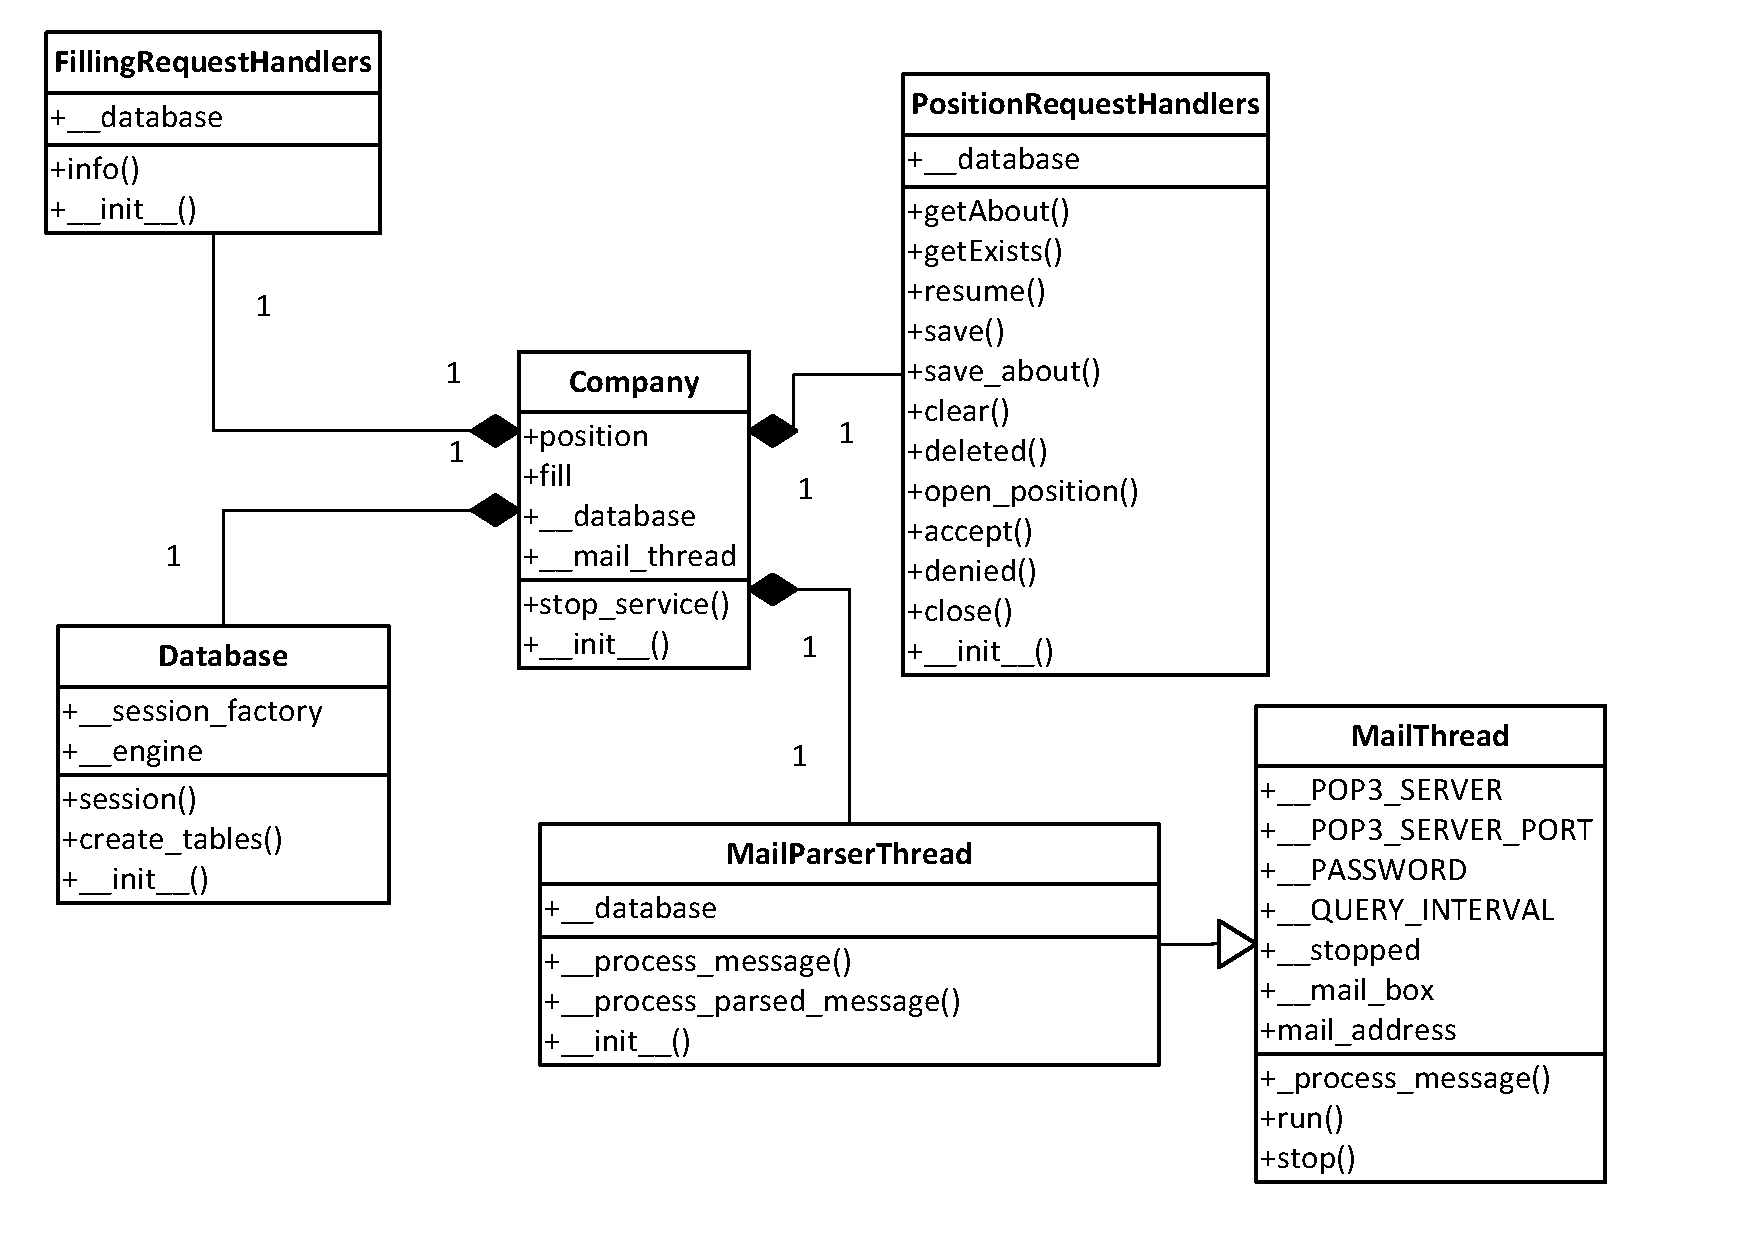
\includegraphics[width=\textwidth]{include/Visio-cmp-uml.pdf}
\caption{Диаграмма классов системы компании-нанимателя}
\label{fig:Visio-cmp-uml}
\end{figure}

Ниже приведена спецификация классов компании-нанимателя.

\textbf{Спецификация классов компании-нанимателя}
\begin{itemize}
\item Database – класс, реализующий прием электронных писем по протоколу POP3.
	\begin{itemize}
	\item create_tables – метод, создающий таблицы из метаданных объектов;
	\item session – метод, сбрасывает все оставшиеся изменения в базу и фиксирует транзакции, в случае неудачи откатывает сессию;
	\end{itemize}	
\item MailThread – класс, реализующий прием электронных писем по протоколу POP3.
	\begin{itemize}
	\item _process_message – метод, переопределяемый в классах-потомках;                                                                   
	\item run – метод запускающий процесс периодической проверки почтового ящика;
	\item stop – метод останавливающий процесс периодической проверки почтового ящика;
	\end{itemize}
\item MailParserThread – класс, унаследованный от MailThread, обрабатывает входящие электронные письма.
	\begin{itemize}
	\item _process_message - метод принимающий письма и получающий из них отправителя и содержимое;     
	\item \underline{ }\underline{ }process_parsed_message - метод обрабатывающий содержимое писем и, в соответствии с полученными данными, изменяющий информацию о доступных вакансиях;
	\end{itemize}
\item FillingRequestHandlers –  класс, выполняющий отправку списка возможных критериев и параметров вакансии в веб-интерфейс.
	\begin{itemize}
	\item info - метод возвращает все возможные списочные параметры, такие как университет, график работы, график командировок, иностранные языки, уровень их знаний и отрасль, в формате JSON;
	\end{itemize}
\item PositionRequestHandlers – класс, выполняющий обработку запросов, поступающих с веб-интерфейса, касающихся создания и обработки вакансий, а также откликов на них.
	\begin{itemize}
	\item getAbout - метод возвращает информацию о компании;
	\item saveAbout - метод сохраняет информацию о компании;
	\item getExists - метод возвращает информацию об открытых вакансиях;
	\item resume - метод возвращает список откликнувшихся кандидатов с названием вакансии, заинтересовавшей их;
	\item save - метод получает данные о вакансии из веб-интерфейса и сохраняет их в базу данных компании;
	\item clear - метод получает идентификатор вакансии и удаляет из базы всю информацию связанную с ней;
	\item deleted - метод получает идентификатор вакансии и удаляет позицию из базы кадрового агентства;
	\item open_position - метод отправляет данные созданной или обновленной вакансии в отраслевую организацию;
	\item accept - метод вызывается при согласии компании перейти к следующему этапу рассмотрения кандидата: изменяется статус отклика, отправляется письмо в отраслевое агентство;
	\item denied - метод вызывается при отказе кандидату в дальнейшем рассмотрении его резюме: изменяется статус отклика в базе, отправляется сообщение в отраслевую организацию;
	\item close - метод закрывает вакансию и посылает в отраслевое агентство сообщение о удалении;
	\end{itemize}	
\end{itemize}

\subsection{Диаграмма классов системы отраслевой организации}
Диаграмма классов для отраслевой организации представлена на рисунке ~\ref{fig:Visio-ia-uml}.


\begin{figure}[ht!]
\centering
 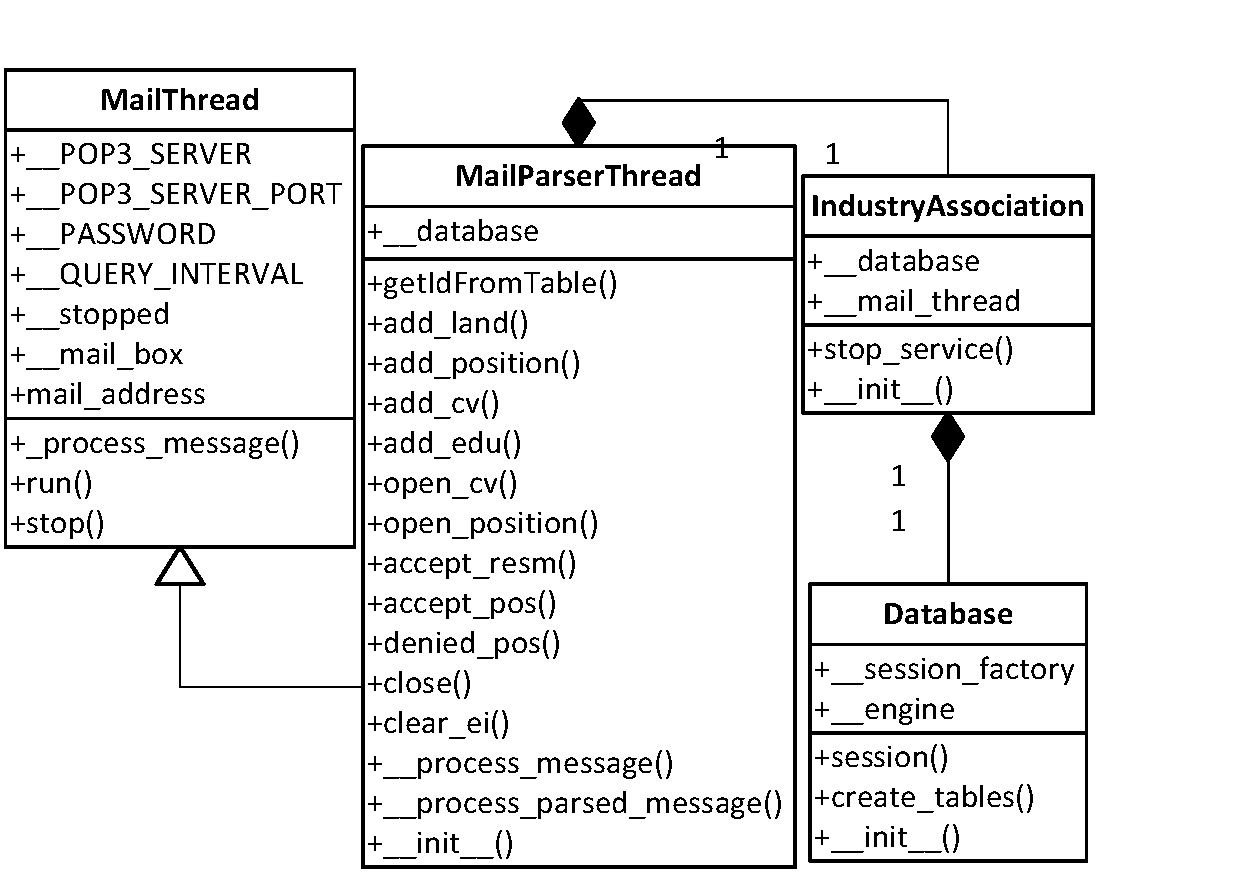
\includegraphics[width=\textwidth]{include/Visio-ia-uml.pdf}
\caption{Диаграмма классов системы отраслевой организации}
\label{fig:Visio-ia-uml}
\end{figure}

Ниже приведена спецификация классов отраслевой организации.

\textbf{Спецификация классов отраслевой организации}
\begin{itemize}
\item Database – класс, реализующий прием электронных писем по протоколу POP3.
	\begin{itemize}
	\item create_tables – метод, создающий таблицы из метаданных объектов;
	\item session – метод, сбрасывает все оставшиеся изменения в базу и фиксирует транзакции, в случае неудачи откатывает сессию;
	\end{itemize}	
\item MailThread – класс, реализующий прием электронных писем по протоколу POP3.
	\begin{itemize}
	\item _process_message – метод, переопределяемый в классах-потомках;                                                                   
	\item run – метод запускающий процесс периодической проверки почтового ящика;
	\item stop – метод останавливающий процесс периодической проверки почтового ящика;
	\end{itemize}
\item MailParserThread – класс, унаследованный от MailThread, обрабатывает входящие электронные письма.
	\begin{itemize}
	\item _process_message - метод принимающий письма и получающий из них отправителя и содержимое;     
	\item \underline{ }\underline{ }process_parsed_message - метод обрабатывающий содержимое писем и, в соответствии с полученными данными, изменяющий информацию о доступных вакансиях;
	\end{itemize}
	
\end{itemize}

\subsubsection{Диаграмма класса, находящегося на узле отраслевой организации, используемого для подбора вакансий}
Диаграмма класса, используемого для подбора вакансий изображена на рисунке ~\ref{fig:Visio-asch-uml}.  
\begin{figure}[ht!]
\centering
 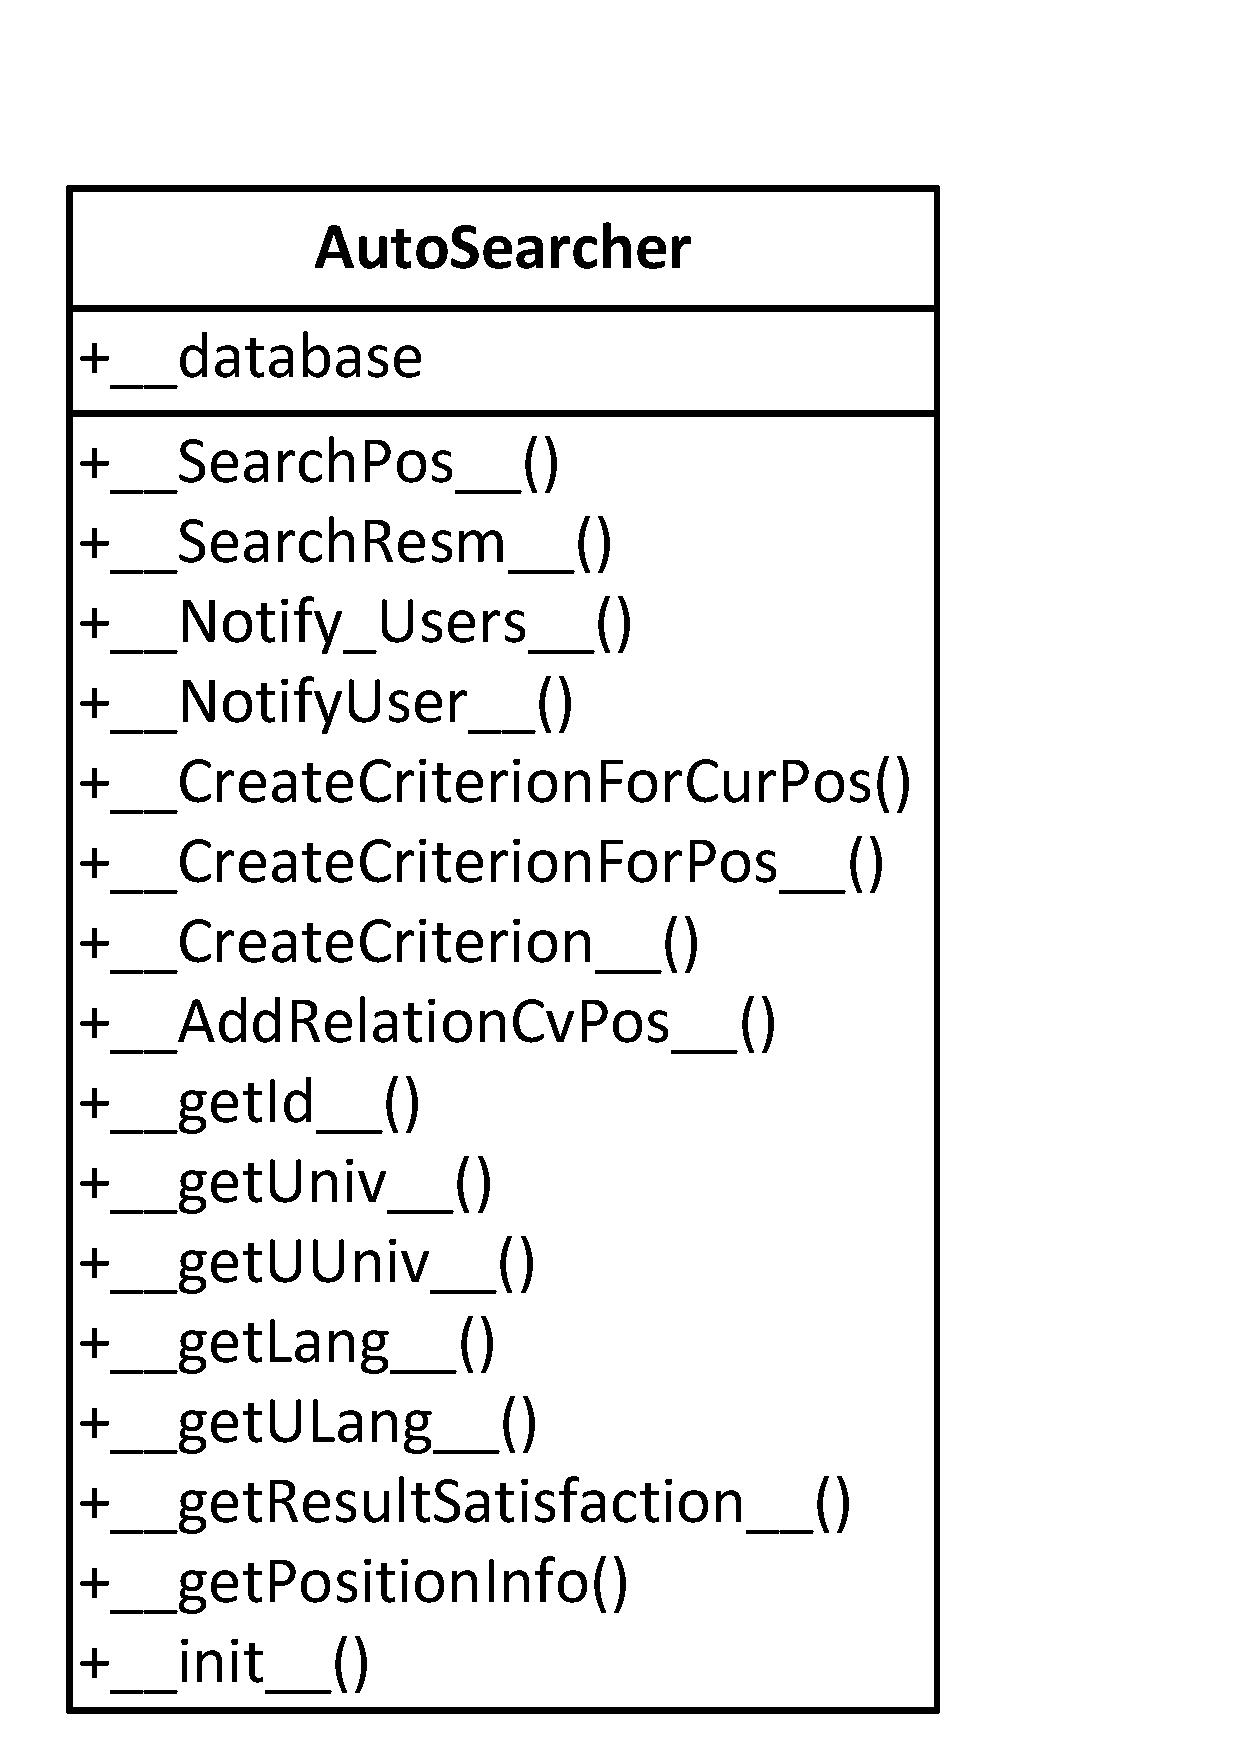
\includegraphics[width=0.5\textwidth]{include/Visio-asch-uml.pdf}
\caption{Диаграмма класса, используемого для подбора вакансий}
\label{fig:Visio-asch-uml}
\end{figure}

Ниже приведена спецификация класса, используемого для подбора вакансий.

\textbf{Спецификация класса, используемого для подбора вакансий}
\begin{itemize}
\item \underline{ }\underline{ }SearchPos\underline{ }\underline{ } – метод, составляющий для кандидатов список вакансий из позиций, для которых критерий схожести с резюме не меньше 0.4;
\item \underline{ }\underline{ }SearchResm\underline{ }\underline{ } – метод, составляющий для вакансии список кандидатов, для которых критерий схожести с резюме не меньше 0.4;
\item \underline{ }\underline{ }Notify_Users\underline{ }\underline{ } – метод, отправляющий письма в по smtp в соответствующие кадровые агентства с идентификаторами подходящих пользователей и описанием вакансии;
\item \underline{ }\underline{ }NotifyUser\underline{ }\underline{ } – метод, отправляющий письмо по smtp в соответствующее кадровое агентство с идентификатором пользователя и описаниями подходящих для него вакансий;
\item \underline{ }\underline{ }CreateCriterionForCurPos – метод, вычисляющий критерий схожести для текущей позиции;
\item \underline{ }\underline{ }CreateCriterionForPos\underline{ }\underline{ } – метод, собирающий все необходимые базы всех резюме и вызывающий метод  \underline{ }\underline{ }CreateCriterionForCurPos для каждого из них и для новой вакансии;
\item \underline{ }\underline{ }CreateCriterion\underline{ }\underline{ } – метод, собирающий все необходимые базы всех вакансий и вызывающий метод  \underline{ }\underline{ }CreateCriterionForCurPos для каждой из них и для нового резюме;
\item \underline{ }\underline{ }AddRelationCvPos\underline{ }\underline{ } – метод, изменяющий статус отклика соискателя на вакансию;
\item \underline{ }\underline{ }getId\underline{ }\underline{ } – метод, получает id строки таблицы по name (только для тех таблиц, в которых данное поле есть);
\item \underline{ }\underline{ }getUniv\underline{ }\underline{ } – метод, получает массив университет и массив специальностей, перечисленных в вакансии;
\item \underline{ }\underline{ }getUUniv\underline{ }\underline{ } – метод, получает массив университет и массив специальностей, перечисленных в резюме;
\item \underline{ }\underline{ }getLang\underline{ }\underline{ } – метод, получает массив иностранных языков и массив уровней подготовки по ним, перечисленных в вакансии 
\item \underline{ }\underline{ }getULang\underline{ }\underline{ } – метод, получает массив иностранных языков и массив уровней подготовки по ним, перечисленных в резюме;
\item \underline{ }\underline{ }getResultSatisfaction\underline{ }\underline{ } – метод, принимающий для сравнения две строки, возвращает true, если отношение совпадающих слов к количеству слов в первой строке больше 0.4;
\item \underline{ }\underline{ }getPositionInfo – метод, формирующий текст - информацию о вакансии для дальнейшей отправки ее в кадровые агентства и просмотра соискателями;

\end{itemize}

\section{Развертывание системы} 
Технические требования к серверам:
Процессор: Pentium III 500 MHz;
ОЗУ: 128 Мбайт;
OC: Linux, Windows, Mac OS;
Программное обеспечение: Python 2.7, SQLAlchemy, CherryPy

На клиентском компьютере должен быть установлен веб-браузер, а разрешение экрана не менее 800x600 точек на дюйм.

\section{Тестирование системы} 
Для проверки работоспособности системы было проведено тестирование функциональных возможностей системы.

\begin{longtable}[ht]{|p{3,5cm}|p{3,5cm}|p{3,5cm}|p{3,5cm}|}
\caption{Результаты тестирования}\label{tab:tab-test-results} \\
\hline
Информация о тесте & Описание теста & Ожидаемый результат  & Результат \\
\hline\hline\endfirsthead
\caption{Результаты тестирования (продолжение)} \\
\hline
Информация о тесте & Описание теста & Ожидаемый результат  & Результат \\
\hline\hline\endhead
\hline
\multicolumn{4}{c}{\textit{Продолжение на следующей странице}}
\endfoot
\endlastfoot
Проверка работы регистрации & Ввод корректных данных & Успешная регистрация в системе & Успешно \\
\hline
Проверка работы регистрации & Ввод зарегистрированного в системе логина& Сообщение, о том, что e-mail уже зарегистрирован & Успешно \\
\hline
Проверка работы регистрации & Незаполненные поля& Сообщение, о том, что некоторые поля пусты & Успешно \\
\hline
Проверка работы авторизации & Ввод верного логина и пароля & Успешный вход в систему & Успешно \\
\hline
Проверка работы авторизации & Ввод незарегистрированного в системе логина или неверного пароля & Сообщение, о ошибке в e-mail или пароле & Успешно \\
\hline
Проверка создания резюме  & Ввод корректных данных & Успешное создание резюме & Успешно \\
\hline
Проверка создания вакансии  & Ввод корректных данных & Успешное создание вакансии & Успешно \\
\hline
Проверка заполнения данных об образовании & Ввод корректных данных & Успешное сохранение данных об образовании & Успешно \\
\hline
Проверка заполнения данных об образовании & Повтор университета и специальности &  Сообщение о дублировании образования & Успешно \\
\hline
Проверка заполнения данных о владении иностранными языками & Ввод корректных данных & Успешное сохранение данных о владении языками & Успешно \\
\hline
Проверка заполнения данных о владении иностранными языками & Повтор наименования языка &  Сообщение о дублировании & Успешно \\
\hline
Проверка создания вакансий  & Ввод корректных данных & Успешное создание вакансий & Успешно \\
\hline
Проверка отправки сообщений отраслевым организациям от компании-нанимателя  & Отправка вакансий для поиска сотрудников & Система отраслевой организации запускает поиск и информирует найденных сотрудников о новой вакансии & Успешно \\
\hline
Проверка отправки сообщений отраслевым организациям от кадрового агентства  & Отправка резюме для поиска вакансий & Система отраслевой организации запускает поиск и информирует сотрудник о подходящих вакансиях & Успешно \\
\hline
Проверка обновления информации & Закрыть вакансию & Система отраслевой организации удаляет вакансию из списка и сигнализирует подписанным пользователям о закрытии указанной заявки & Успешно \\
\hline
\end{longtable}



























%


\backmatter %% Здесь заканчивается нумерованная часть документа и начинаются ссылки и

\Conclusion % заключение к отчёту
В результате проделанной работы:
\begin{enumerate}
\item проведен анализ предметной области; 
\item определены требования к системе;
\item спроектирована структура субъектов РСОИ и протокол их взаимодействия;
\item реализована логика работы узлов системы.
\end{enumerate}
Разработанная система содержит субъекты трех типов:
\begin{enumerate}
\item компания-наниматель;
\item кадровое-агентство;
\item отраслевая организация.
\end{enumerate}

Эти системы являются независимыми и взаимодействуют по открытым каналам связи по разработанному протоколу.

В качестве усовершенствования проекта можно предложить буферизацию входящих сообщений, а также более детально рассмотреть вопросы отказоустойчивости системы и восстановления работоспособности системы после сбоев.

%%% Local Variables: 
%%% mode: latex
%%% TeX-master: "rpz"
%%% End: 


% % Список литературы при помощи BibTeX
% Юзать так:
%
% pdflatex rpz
% bibtex rpz
% pdflatex rpz

\bibliographystyle{gost780u}
\bibliography{rpz}

\begin{thebibliography}{9}

\bibitem{RSOI} 
  Э. Таненбаум, М. ван Стеен. 
  \emph{ Распределенные системы. Принципы и парадигмы}.
  — СПб.: Питер, 2003. — 877 с: ил.
\bibitem{UML}
	Буч Г., Рамбо Д., Якобсон И.
\emph{Язык UML. Руководство пользователя}. 
2-е изд.: Пер. с англ. Мухин Н. – М.: ДМК Пресс. – 496 с.: ил.
\bibitem{STUDY}
	Крищенко, В. А.
\emph{Распределенные системы обработки информации. Указания по курсовому проектированию}.
2011.
\bibitem{Python}
	Dive Into Python 3, Mark Pilgrim, http://getpython3.com/diveintopython3/
\bibitem{CherryPy}
	Team, CherryPy. CherryPy Documentation. — http://docs.cherrypy.org/
stable/intro/index.html.

\end{thebibliography}

%\appendix   % Тут идут приложения

%\include{90-appendix1}
%\include{91-appendix2}

\end{document}
%%% Local Variables:
%%% mode: latex
%%% TeX-master: t
%%% End:
